

\setcounter{chapter}{4}

\chapter{直积、半直积与阿贝尔群}

本章我们考虑从较小群构造较大群的两种较容易的方法，即直积与半直积的概念。这使我们能够陈述有限生成阿贝尔群基本定理，它特别完全分类了所有有限阿贝尔群。

\section{直积}

我们从有限个和可数个群的直积的定义开始（任意一族群的直积在习题中考虑）。

\begin{definition}
（1）群 \(G_1, G_2, \ldots, G_n\)（运算分别为 \(*_1, *_2, \ldots, *_n\)）的\textbf{直积} \(G_1 \times G_2 \times \cdots \times G_n\) 是 \(n\) 元组 \((g_1, g_2, \ldots, g_n)\)（其中 \(g_i \in G_i\)）的集合，其运算按分量定义：
\[
(g_1, g_2, \ldots, g_n) * (h_1, h_2, \ldots, h_n) = (g_1 *_1 h_1,\ g_2 *_2 h_2,\ \ldots,\ g_n *_n h_n).
\]
（2）类似地，群 \(G_1, G_2, \ldots\)（运算分别为 \(*_1, *_2, \ldots\)）的\textbf{直积} \(G_1 \times G_2 \times \cdots\) 是序列 \((g_1, g_2, \ldots)\)（其中 \(g_i \in G_i\)）的集合，其运算按分量定义：
\[
(g_1, g_2, \ldots) * (h_1, h_2, \ldots) = (g_1 *_1 h_1,\ g_2 *_2 h_2,\ \ldots).
\]
\end{definition}

尽管直积各因子中的运算可能不同，我们照例把所有抽象群都写成乘法的，于是上面的（1）中的运算简单地变成
\[
(g_1, g_2, \ldots, g_n)(h_1, h_2, \ldots, h_n) = (g_1h_1,\ g_2h_2,\ \ldots,\ g_nh_n).
\]

\begin{example}
（1）\(\mathbb{R}^n = \mathbb{R} \times \mathbb{R} \times \cdots \times \mathbb{R}\)（\(n\) 个因子）是加法下的阿贝尔群，运算为
\[
(a_1, a_2, \ldots, a_n) + (b_1, b_2, \ldots, b_n) = (a_1 + b_1,\ a_2 + b_2,\ \ldots,\ a_n + b_n).
\]

（2）为说明构成直积的群（及其相应的运算）可以完全一般，设 \(G_1 = \mathbb{Z}\)、\(G_2 = S_3\)、\(G_3 = GL_2(\mathbb{R})\)，其中群运算分别是加法、复合和矩阵乘法。则 \(G_1 \times G_2 \times G_3\) 中的运算定义为
\[
\left(n,\ \sigma,\ \begin{pmatrix} a & b \\ c & d \end{pmatrix}\right)\left(m,\ \tau,\ \begin{pmatrix} p & q \\ r & s \end{pmatrix}\right) = \left(n+m,\ \sigma \circ \tau,\ \begin{pmatrix} ap+br & aq+bs \\ cp+dr & cq+ds \end{pmatrix}\right).
\]
\end{example}

\begin{proposition}\label{pro:5.1}
若 \(G_1, \ldots, G_n\) 是群，则它们的直积是阶为 \(|G_1||G_2|\cdots|G_n|\) 的群（若某个 \(G_i\) 无限，则直积也无限）。
\end{proposition}

\begin{proof}
设 \(G = G_1 \times G_2 \times \cdots \times G_n\). 群公理对 \(G\) 成立的证明很直接，因为每条公理都是它在每个因子 \(G_i\) 中成立这一事实的推论，且 \(G\) 上的运算按分量定义。例如，结合律验证如下：设 \((a_1, a_2, \ldots, a_n), (b_1, b_2, \ldots, b_n), (c_1, c_2, \ldots, c_n) \in G\). 则
\[
\begin{aligned}
&(a_1, a_2, \ldots, a_n)\left[(b_1, b_2, \ldots, b_n)(c_1, c_2, \ldots, c_n)\right] \\
&=(a_1, a_2, \ldots, a_n)(b_1c_1,\ b_2c_2,\ \ldots,\ b_nc_n) \\
&=(a_1(b_1c_1),\ a_2(b_2c_2),\ \ldots,\ a_n(b_nc_n)) \\
&=((a_1b_1)c_1,\ (a_2b_2)c_2,\ \ldots,\ (a_nb_n)c_n) \\
&=\left[(a_1, a_2, \ldots, a_n)(b_1, b_2, \ldots, b_n)\right](c_1, c_2, \ldots, c_n),
\end{aligned}
\]
其中第三步用了每个分量中的结合律。直积是群的其余验证类似：\(G\) 的单位元是 \((1, 1, \ldots, 1)\)，其中 \(1\) 是每个 \(G_i\) 的单位元；\((g_1, g_2, \ldots, g_n)\) 的逆元是 \((g_1^{-1}, g_2^{-1}, \ldots, g_n^{-1})\)，其中 \(g_i^{-1}\) 是 \(g_i\) 在 \(G_i\) 中的逆元。\(G\) 的阶的公式是显然的。
\end{proof}

若重新排列直积的因子，所得的直积与原直积同构（参见习题 7）。

下一个命题表明直积 \(G_1 \times G_2 \times \cdots \times G_n\) 含有每个 \(G_i\) 的一个同构复制。可以把这些特定的复制看作直积的“坐标轴”，因为对于 \(\mathbb{R} \times \mathbb{R}\)，它们与 \(x\) 轴和 \(y\) 轴重合。但要注意，不要把“坐标轴”看作直积中群 \(G_i\) 的唯一的复制。例如在 \(\mathbb{R} \times \mathbb{R}\) 中，过原点的任何直线都是同构于 \(\mathbb{R}\) 的子群（且 \(\mathbb{R} \times \mathbb{R}\) 有无穷多对作为坐标轴的直线，即给定坐标系的任意旋转）。命题的第二部分表明存在到每个分量上的投影同态。

\begin{proposition}\label{pro:5.2}
设 \(G_1, G_2, \ldots, G_n\) 是群，\(G = G_1 \times \cdots \times G_n\) 是它们的直积。

（1）对每个固定的 \(i\)，\(G\) 中那些在第 \(j\) 个位置（对所有 \(j \neq i\)）取 \(G_j\) 的单位元、在第 \(i\) 个位置取 \(G_i\) 的任意元素的元素构成的集合是 \(G\) 的一个同构于 \(G_i\) 的子群：
\[
G_i \cong \{(1, 1, \ldots, 1, g_i, 1, \ldots, 1) \mid g_i \in G_i\}
\]
（这里 \(g_i\) 出现在第 \(i\) 个位置）。若把 \(G_i\) 与这个子群等同，则 \(G_i \trianglelefteq G\) 且
\[
G/G_i \cong G_1 \times \cdots \times G_{i-1} \times G_{i+1} \times \cdots \times G_n.
\]

（2）对每个固定的 \(i\)，定义 \(\pi_i : G \to G_i\) 为
\[
\pi_i((g_1, g_2, \ldots, g_n)) = g_i.
\]
则 \(\pi_i\) 是满同态，且
\[
\ker \pi_i = \{(g_1, \ldots, g_{i-1}, 1, g_{i+1}, \ldots, g_n) \mid g_j \in G_j \text{ 对所有 } j \neq i\} \cong G_1 \times \cdots \times G_{i-1} \times G_{i+1} \times \cdots \times G_n
\]
（这里 \(1\) 出现在第 \(i\) 个位置）。

（3）在（1）的等同下，若 \(x \in G_i\)、\(y \in G_j\)（\(i \neq j\)），则
\[
xy = yx.
\]
\end{proposition}

\begin{proof}
（1）由于 \(G\) 中的运算按分量定义，由子群判别法容易得出 \(\{(1, 1, \ldots, 1, g_i, 1, \ldots, 1) \mid g_i \in G_i\}\) 是 \(G\) 的子群。此外，映射 \(g_i \mapsto (1, 1, \ldots, 1, g_i, 1, \ldots, 1)\) 是 \(G_i\) 与这个子群的一个同构。把 \(G_i\) 与 \(G\) 中这个同构复制等同。

为证（1）余下的部分，考虑由
\[
\varphi(g_1, g_2, \ldots, g_n) = (g_1, \ldots, g_{i-1}, g_{i+1}, \ldots, g_n)
\]
定义的映射 \(\varphi : G \to G_1 \times \cdots \times G_{i-1} \times G_{i+1} \times \cdots \times G_n\)（即 \(\varphi\) 抹去 \(G\) 的第 \(i\) 个分量）。\(\varphi\) 是同态，因为
\[
\begin{aligned}
\varphi((g_1, \ldots, g_n)(h_1, \ldots, h_n)) &= \varphi((g_1h_1, \ldots, g_nh_n)) \\
&= (g_1h_1, \ldots, g_{i-1}h_{i-1}, g_{i+1}h_{i+1}, \ldots, g_nh_n) \\
&= (g_1, \ldots, g_{i-1}, g_{i+1}, \ldots, g_n)(h_1, \ldots, h_{i-1}, h_{i+1}, \ldots, h_n) \\
&= \varphi((g_1, \ldots, g_n))\varphi((h_1, \ldots, h_n)).
\end{aligned}
\]
由于第 \(j\) 个位置的元素对所有 \(j\) 都可任意取 \(G_j\) 的元素，\(\varphi\) 是满射。此外，
\[
\ker \varphi = \{(g_1, \ldots, g_n) \mid g_j = 1 \text{ 对所有 } j \neq i\} = G_i.
\]
这证明 \(G_i\) 是 \(G\) 的正规子群（特别地，再次证明这个 \(G_i\) 的复制是子群），且第一同构定理给出（1）的最后一个论断。

（2）中 \(\pi_i\) 是满同态、且其核是所述子群的论证与（1）非常相似，细节留给读者。（3）中若 \(x = (1, \ldots, 1, g_i, 1, \ldots, 1)\)、\(y = (1, \ldots, 1, g_j, 1, \ldots, 1)\)，其中所示元素分别出现在位置 \(i, j\)，则
\[
xy = (1, \ldots, 1, g_i, 1, \ldots, 1, g_j, 1, \ldots, 1) = yx
\]
（记号的选择使 \(i < j\)）。完成证明。
\end{proof}

这个命题的推广见习题 2。

我们将继续把命题 (1) 中描述的“坐标轴”子群与其同构复制 \(G_i\) 等同。第 \(i\) 个这样的子群常称为 \(G\) 的第 \(i\) 个\textbf{分量}或第 \(i\) 个\textbf{因子}。例如，当我们要在 \(Z_n \times Z_m\) 中计算时，可以让 \(x\) 是第一个因子的生成元、\(y\) 是第二个因子的生成元，并把 \(Z_n \times Z_m\) 的元素写成 \(x^a y^b\) 的形式。这用 \(x\) 和 \(y\) 替换了形式有序对 \((x, 1)\) 和 \((1, y)\)（于是 \(x^a y^b\) 替换 \((x^a, y^b)\)）。

\begin{example}
（1）在命题 \ref{pro:5.2} 的记号下，由（3）可得若 \(x_i \in G_i\)（\(1 \leq i \leq n\)），则对所有 \(k \in \mathbb{Z}\) 有
\[
(x_1 x_2 \cdots x_n)^k = x_1^k x_2^k \cdots x_n^k.
\]
由于 \(x_1x_2\cdots x_n\) 的阶是使对所有 \(i\) 有 \(x_i^k = 1\) 的最小正整数 \(k\)，我们看到
\[
|x_1x_2\cdots x_n| = \operatorname{lcm}(|x_1|, |x_2|, \ldots, |x_n|)
\]
（其中该阶无限当且仅当某个 \(x_i\) 的阶无限）。

（2）设 \(p\) 是素数，对 \(n \in \mathbb{Z}^+\) 考虑
\[
E_{p^n} = Z_p \times Z_p \times \cdots \times Z_p \quad (n \text{ 个因子}).
\]
这个群是 \(p^n\) 阶阿贝尔群，具有 4.4 节习题中描述的性质 \(px = 1\)（对所有 \(x\)）。\(E_{p^n}\) 是 \(p^n\) 阶\textbf{初等阿贝尔群}。

（3）对素数 \(p\)，我们证明 \(p^2\) 阶初等阿贝尔群 \(E = E_{p^2}\) 恰有 \(p+1\) 个 \(p\) 阶子群（特别地，比显然的两个要多）。由于 \(E\) 的每个非单位元都是 \(p\) 阶的，每个非单位元生成 \(E\) 的一个 \(p\) 阶循环子群。由拉格朗日定理，不同的 \(p\) 阶子群交为单位元。于是 \(E\) 的 \(p^2 - 1\) 个非单位元被划分成大小为 \(p-1\) 的子集（即每个这样的子集由某个 \(p\) 阶子群的非单位元组成）。因此必有
\[
\frac{p^2 - 1}{p - 1} = p + 1
\]
个 \(p\) 阶子群。当 \(p = 2\) 时，\(E\) 是克莱因四元群，我们已经看到它有 3 个 2 阶子群（另见习题 10 和 11）。
\end{example}

\subsection*{习题}

\begin{enumerate}
\item 证明直积的中心是中心的直积：
\[
Z(G_1 \times G_2 \times \cdots \times G_n) = Z(G_1) \times Z(G_2) \times \cdots \times Z(G_n).
\]
由此推出群的直积是阿贝尔群当且仅当每个因子都是阿贝尔群。

\item 设 \(G_1, G_2, \ldots, G_n\) 是群，\(G = G_1 \times \cdots \times G_n\). 设 \(I\) 是 \(\{1, \ldots, n\}\) 的非空真子集，\(J = \{1, \ldots, n\} - I\). 定义 \(G_I\) 为 \(G\) 中那些对所有 \(j \in J\) 在第 \(j\) 个位置取 \(G_j\) 的单位元的元素组成的集合。

（a）证明 \(G_I\) 同构于群 \(G_i\)（\(i \in I\)）的直积。

（b）证明 \(G_I\) 是 \(G\) 的正规子群，且 \(G/G_I \cong G_J\).

（c）证明 \(G \cong G_I \times G_J\).

\item 在上一习题的记号下，设 \(I\) 和 \(K\) 是 \(\{1, 2, \ldots, n\}\) 的任意不交非空子集，\(G_I\) 和 \(G_K\) 是上面定义的 \(G\) 的子群。证明对所有 \(x \in G_I\) 和所有 \(y \in G_K\) 有 \(xy = yx\).

\item 设 \(A\) 和 \(B\) 是有限群，\(p\) 是素数。证明 \(A \times B\) 的任意西罗 \(p\)-子群都形如 \(P \times Q\)，其中 \(P \in \operatorname{Syl}_p(A)\)、\(Q \in \operatorname{Syl}_p(B)\). 证明 \(n_p(A \times B) = n_p(A)n_p(B)\). 把这两个结果推广到任意有限个有限群的直积（于是直积的西罗 \(p\)-子群个数是各因子西罗 \(p\)-子群个数的乘积）。

\item 给出 \(Q_8 \times Z_4\) 的一个非正规子群（注意每个因子的每个子群都正规）。

\item 证明 \(Q_8 \times E_{2^n}\) 的所有子群都正规。

\item 设 \(G_1, G_2, \ldots, G_n\) 是群，\(\sigma\) 是 \(S_n\) 的固定元素。证明由
\[
\varphi_\sigma(g_1, g_2, \ldots, g_n) = (g_{\sigma^{-1}(1)}, g_{\sigma^{-1}(2)}, \ldots, g_{\sigma^{-1}(n)})
\]
定义的映射 \(\varphi_\sigma : G_1 \times \cdots \times G_n \to G_{\sigma^{-1}(1)} \times \cdots \times G_{\sigma^{-1}(n)}\) 是同构（于是改变直积中因子的顺序不改变同构类型）。

\item 设 \(G_1 = G_2 = \cdots = G_n = G\)，\(\bar{G} = G_1 \times \cdots \times G_n\). 在上一习题的记号下证明 \(\varphi_\sigma \in \operatorname{Aut}(\bar{G})\). 还证明映射 \(\sigma \mapsto \varphi_\sigma\) 是 \(S_n\) 到 \(\operatorname{Aut}(\bar{G})\) 的单同态（特别地，\(\varphi_{\sigma_1} \circ \varphi_{\sigma_2} = \varphi_{\sigma_1\sigma_2}\)）。用记号来说这之所以是一个同态，是因为若 \(e_i\) 是第 \(i\) 个位置为 1、其余为 0 的 \(n\) 元组（\(1 \leq i \leq n\)），则 \(S_n\) 通过 \(\sigma \cdot e_i = e_{\sigma(i)}\) 作用于 \(\{e_1, \ldots, e_n\}\)；这是一个左群作用。若 \(n\) 元组 \((g_1, \ldots, g_n)\) 用 \(g_1e_1 + \cdots + g_ne_n\) 表示，则这个在 \(\{e_1, \ldots, e_n\}\) 上的左群作用通过
\[
\sigma \cdot (g_1e_1 + g_2e_2 + \cdots + g_ne_n) = g_1e_{\sigma(1)} + g_2e_{\sigma(2)} + \cdots + g_ne_{\sigma(n)}
\]
延拓为和上的左群作用。右端 \(e_{\sigma(i)}\) 的系数是 \(g_i\)，故 \(e_i\) 的系数是 \(g_{\sigma^{-1}(i)}\). 于是右端可以改写为 \(g_{\sigma^{-1}(1)}e_1 + g_{\sigma^{-1}(2)}e_2 + \cdots + g_{\sigma^{-1}(n)}e_n\)，这恰好是附着于 \(n\) 元组 \((g_{\sigma^{-1}(1)}, g_{\sigma^{-1}(2)}, \ldots, g_{\sigma^{-1}(n)})\) 的和。换句话说，“位置向量” \(e_1, \ldots, e_n\) 的任意置换（固定其系数）等同于系数上的逆置换（固定 \(e_i\)）。若在 \(\varphi_\sigma\) 的定义中用 \(\sigma\) 代替 \(\sigma^{-1}\)，则映射 \(\sigma \mapsto \varphi_\sigma\) 不一定是同态——它对应于右群作用。

\item 设对所有 \(i\)，\(G_i\) 是域 \(F\)，用前一习题证明每行每列恰有一个 1 的 \(n \times n\) 矩阵的集合是 \(GL_n(F)\) 的一个同构于 \(S_n\) 的子群（这些矩阵称为\textbf{置换矩阵}，因为它们只是置换 \(n\) 维向量空间 \(F \times F \times \cdots \times F\) 的标准基 \(e_1, \ldots, e_n\)（如上））。

\item 设 \(p\) 是素数。设 \(A\) 和 \(B\) 是两个 \(p\) 阶循环群，生成元分别为 \(x\) 和 \(y\)。令 \(E = A \times B\)，故 \(E\) 是 \(p^2\) 阶初等阿贝尔群：\(E = E_{p^2}\). 证明 \(E\) 的不同的 \(p\) 阶子群是
\[
\langle x \rangle,\quad \langle xy \rangle,\quad \langle x^2 y \rangle,\quad \ldots,\quad \langle x^{p-1}y \rangle,\quad \langle y \rangle
\]
（注意共有 \(p+1\) 个）。

\item 设 \(p\) 是素数，\(n \in \mathbb{Z}^+\). 用取整函数求初等阿贝尔群 \(E_{p^n}\) 中 \(p\) 阶子群个数的公式。

\item 设 \(A\) 和 \(B\) 是群。假设 \(Z(A)\) 含有子群 \(Z_1\)，\(Z(B)\) 含有子群 \(Z_2\)，且 \(Z_1 \cong Z_2\). 设这个同构由映射 \(x_i \mapsto y_i\) 给出（对所有 \(x_i \in Z_1\)）。\(A\) 和 \(B\) 的\textbf{中心积}是商
\[
(A \times B)/Z, \quad \text{其中 } Z = \{(x_i,\ y_i^{-1}) \mid x_i \in Z_1\},
\]
记作 \(A * B\)——它不唯一，因为它依赖于 \(Z_1, Z_2\) 以及它们之间的同构。（把 \(A * B\) 想成 \(A\) 与 \(B\) 的直积，通过把每个 \(x_i \in Z_1\) 与对应的 \(y_i \in Z_2\) 等同起来而“坍缩”。）

（a）证明 \(A\) 和 \(B\) 在商群 \(A * B\) 中的像分别同构于 \(A\) 和 \(B\)，且这些像交为一个同构于 \(Z_1\) 的中心子群。求 \(|A * B|\).

（b）设 \(Z_4 = \langle x \rangle\). 设 \(D_8 = \langle r, s \rangle\)、\(Q_8 = \langle i, j \rangle\) 由通常的生成元与关系给出。设 \(Z_4 * D_8\) 是把 \(x^2\) 与 \(r^2\) 等同的 \(Z_4\) 与 \(D_8\) 的中心积（即 \(Z_1 = \langle x^2 \rangle\)、\(Z_2 = \langle r^2 \rangle\)，同构是 \(x^2 \mapsto r^2\)），设 \(Z_4 * Q_8\) 是把 \(x^2\) 与 \(-1\) 等同的 \(Z_4\) 与 \(Q_8\) 的中心积。证明 \(Z_4 * D_8 \cong Z_4 * Q_8\).

\item 给出上一习题中构造的群 \(Z_4 * D_8\) 和 \(Z_4 * Q_8\) 的生成元与关系。

\item 设 \(G = A_1 \times A_2 \times \cdots \times A_n\)，并对每个 \(i\) 设 \(B_i\) 是 \(A_i\) 的正规子群。证明 \(B_1 \times B_2 \times \cdots \times B_n \trianglelefteq G\)，且
\[
(A_1 \times \cdots \times A_n)/(B_1 \times \cdots \times B_n) \cong (A_1/B_1) \times (A_2/B_2) \times \cdots \times (A_n/B_n).
\]

\noindent 下面这个习题描述任意一族群的直积。任意一族集合的笛卡尔积的术语见附录。

\item 设 \(I\) 是任意非空指标集，对每个 \(i \in I\)，\((G_i, *_i)\) 是群。群 \(G_i\)（\(i \in I\)）的\textbf{直积}是集合 \(G = \prod_{i \in I} G_i\)（各 \(G_i\) 的笛卡尔积），其二元运算定义如下：若 \(\prod a_i\) 和 \(\prod b_i\) 是 \(G\) 的元素，则它们在 \(G\) 中的乘积为
\[
\prod a_i \cdot \prod b_i = \prod (a_i *_i b_i),
\]
即直积中的群运算按分量定义。

（a）证明这个二元运算是良定义的、结合的。

（b）证明元素 \(\prod 1_i\) 满足 \(G\) 的单位元公理，其中 \(1_i\) 是 \(G_i\) 的单位元（对所有 \(i\)）。

（c）证明元素 \(\prod a_i^{-1}\) 是 \(\prod a_i\) 的逆元，其中每个分量元素 \(a_i\) 的逆元在群 \(G_i\) 中取。

由此得出直积是群。（注意若 \(I = \{1, 2, \ldots, n\}\)，这个直积的定义与正文中的 \(n\) 元组定义相同。）

\item 陈述并证明命题 \ref{pro:5.2} 对任意直积的推广。

\item 设 \(I\) 是任意非空指标集，对每个 \(i \in I\)，\(G_i\) 是群。群 \(G_i\) 的\textbf{受限直积}或\textbf{直和}是直积中除有限多个分量外都为单位元的元素组成的集合，即所有这样的元素 \(\prod a_i \in \prod_{i \in I} G_i\)：除 \(I\) 中有限多个 \(i\) 外有 \(a_i = 1_i\).

（a）证明受限直积是直积的子群。

（b）证明受限直积在直积中正规。

（c）设 \(I = \mathbb{Z}^+\)，\(p_i\) 是第 \(i\) 个素数。证明：若对所有 \(i \in \mathbb{Z}^+\) 有 \(G_i = \mathbb{Z}/p_i\mathbb{Z}\)，则受限直积的每个元素都是有限阶的，而 \(\prod_{i \in \mathbb{Z}^+} G_i\) 有无穷阶元素。证明在这个例子中受限直积是直积的挠子群（参见第 2.1 节习题 6）。

\item 在 (a) 到 (e) 中各给出一个具有指定性质的群的例子：

（a）每个元素阶为 1 或 2 的无限群；

（b）每个元素都是有限阶的无限群，但对每个正整数 \(n\) 都有 \(n\) 阶元素；

（c）含有无穷阶元素和 2 阶元素的群；

（d）一个群 \(G\)，使得每个有限群都同构于 \(G\) 的某个子群；

（e）一个非平凡群 \(G\)，使得 \(G \cong G \times G\).
\end{enumerate}

\section{有限生成阿贝尔群基本定理}

\begin{definition}
（1）群 \(G\) 称为\textbf{有限生成的}，若存在 \(G\) 的有限子集 \(A\) 使 \(G = \langle A \rangle\).

（2）对每个 \(r \geq 0\)，令 \(\mathbb{Z}^r = \mathbb{Z} \times \mathbb{Z} \times \cdots \times \mathbb{Z}\)（\(r\) 个因子，约定 \(\mathbb{Z}^0 = 1\)）。群 \(\mathbb{Z}^r\) 称为秩为 \(r\) 的\textbf{自由阿贝尔群}。
\end{definition}

注意任何有限群 \(G\) 自然是有限生成的：只需取 \(A = G\) 作为生成元集合。又 \(\mathbb{Z}^n\) 由 \(e_1, e_2, \ldots, e_n\) 有限生成，其中 \(e_i\) 是第 \(i\) 个位置为 1、其余为 0 的 \(n\) 元组。现在我们可以陈述（有限生成）阿贝尔群的基本分类定理。

\begin{theorem}[有限生成阿贝尔群基本定理]\label{thm:5.3}
设 \(G\) 是有限生成阿贝尔群。则

\begin{enumerate}[label=(\arabic*)]
\item
\[
G \cong \mathbb{Z}^r \times Z_{n_1} \times Z_{n_2} \times \cdots \times Z_{n_s},
\]
其中整数 \(r, n_1, n_2, \ldots, n_s\) 满足下列条件：

（a）\(r \geq 0\) 且对所有 \(j\) 有 \(n_j \geq 2\)；

（b）\(n_{i+1} \mid n_i\)（\(1 \leq i \leq s-1\)）。

\item （1）中的表达式是唯一的：若 \(G \cong \mathbb{Z}^t \times Z_{m_1} \times Z_{m_2} \times \cdots \times Z_{m_u}\)，其中 \(t, m_1, m_2, \ldots, m_u\) 满足（a）和（b）（即 \(t \geq 0\)、对所有 \(j\) 有 \(m_j \geq 2\)，且 \(m_{i+1} \mid m_i\)（\(1 \leq i \leq u-1\)）），则 \(t = r\)、\(u = s\)，且对所有 \(i\) 有 \(m_i = n_i\).
\end{enumerate}
\end{theorem}

\begin{proof}
我们将在 12.1 节把本定理作为更一般的分类定理的推论导出。对有限群，我们将在 6.1 节末给出另一个证明。
\end{proof}

\begin{definition}
定理 \ref{thm:5.3} 中的整数 \(r\) 称为 \(G\) 的\textbf{自由秩}或\textbf{贝蒂数}，整数 \(n_1, n_2, \ldots, n_s\) 称为 \(G\) 的\textbf{不变因子}。定理 \ref{thm:5.3}(1) 中对 \(G\) 的描述称为 \(G\) 的\textbf{不变因子分解}。
\end{definition}

定理 \ref{thm:5.3} 断言阿贝尔群的自由秩和（有序的）不变因子表是唯一确定的，因此两个有限生成阿贝尔群同构当且仅当它们有相同的自由秩和相同的不变因子表。注意有限生成阿贝尔群是有限群当且仅当它的自由秩为零。

有限阿贝尔群的阶恰好是它的不变因子之积（由命题 \ref{pro:5.1}）。若 \(G\) 是有限阿贝尔群，不变因子为 \(n_1, n_2, \ldots, n_s\)，其中 \(n_{i+1} \mid n_i\)（\(1 \leq i \leq s-1\)），则称 \(G\) 为 \textbf{\((n_1, n_2, \ldots, n_s)\) 型}的。

定理 \ref{thm:5.3} 给出了列出给定阶的所有有限阿贝尔群的有效方法。也就是说，为求出（在同构意义下）给定阶 \(n\) 的所有阿贝尔群，必须求出所有满足下列条件的整数有限序列 \(n_1, n_2, \ldots, n_s\)：

\begin{enumerate}[label=(\arabic*)]
\item 对所有 \(j \in \{1, 2, \ldots, s\}\) 有 \(n_j \geq 2\)；
\item \(n_{i+1} \mid n_i\)（\(1 \leq i \leq s-1\)）；
\item \(n_1n_2\cdots n_s = n\).
\end{enumerate}

定理 \ref{thm:5.3} 表明这样的序列的集合与 \(n\) 阶有限阿贝尔群的同构类的集合之间存在双射（其中每个序列对应一个有限阿贝尔群的不变因子表）。

在说明如何对具体的 \(n\) 值求出所有这样的序列之前，我们作一些一般性的评注。首先注意 \(n_1 \geq n_2 \geq \cdots \geq n_s\)，故 \(n_1\) 是最大的不变因子。又由性质（3），每个 \(n_i\) 整除 \(n\)。若 \(p\) 是 \(n\) 的任意素因子，则由（3）知 \(p\) 必整除某个 \(n_i\)。于是由（2），\(p\) 也整除所有 \(j \geq i\) 的 \(n_j\)。由此可得
\begin{center}
\(n\) 的每个素因子必整除第一个不变因子 \(n_1\).
\end{center}
特别地，若 \(n\) 是互不相同素数（都是一次幂）的乘积\footnote{这样的整数称为\textbf{无平方因子的}，因为它们不被任何大于 1 的平方整除。}，我们看到 \(n \mid n_1\)，故 \(n = n_1\)。这证明了若 \(n\) 无平方因子，则 \(n\) 阶阿贝尔群只有一种可能的不变因子表（即表 \(n_1 = n\)）：

\begin{corollary}\label{cor:5.4}
若 \(n\) 是互不相同素数的乘积，则在不计同构的意义下，唯一的 \(n\) 阶阿贝尔群是 \(n\) 阶循环群 \(Z_n\).
\end{corollary}

把 \(n\) 分解成素数幂是确定 \(n\) 阶阿贝尔群所有可能不变因子表的第一步。

\begin{example}
设 \(n = 180 = 2^2 \cdot 3^2 \cdot 5\). 如上所述必有 \(2 \cdot 3 \cdot 5 \mid n_1\)，故 \(n_1\) 的可能取值是
\[
n_1 = 2^2 \cdot 3^2 \cdot 5,\quad 2^2 \cdot 3 \cdot 5,\quad 2 \cdot 3^2 \cdot 5,\quad \text{或 } 2 \cdot 3 \cdot 5.
\]
对其中每个都必须求出所有可能的 \(n_2\)（满足 \(n_2 \mid n_1\) 且 \(n_1n_2 \mid n\)）。对每个得到的数对 \(n_1, n_2\) 都必须求出所有可能的 \(n_3\)，如此继续，直到得到满足（1）至（3）的表。

例如，若 \(n_1 = 2 \cdot 3^2 \cdot 5\)，则唯一整除 \(n_1\) 且使 \(n_1n_2\) 整除 \(n\) 的数 \(n_2\) 是 \(n_2 = 2\). 此时 \(n_1n_2 = n\)，故这个表是完整的：\(2 \cdot 3^2 \cdot 5,\ 2\). 与这个表对应的阿贝尔群是 \(Z_{90} \times Z_2\).

若 \(n_1 = 2 \cdot 3 \cdot 5\)，则 \(n_2\) 的候选值只有 \(n_2 = 2, 3\) 或 6. 若 \(n_2 = 2\) 或 3，则由于 \(n_3 \mid n_2\)，必有 \(n_3 = n_2\)（且由性质（3）表中必有第三项）。这导致矛盾，因为 \(n_1n_2n_3\) 将分别被 \(2^3\) 或 \(3^3\) 整除，而 \(n\) 不被这两者中任何一个整除。因此第一个项为 \(2 \cdot 3 \cdot 5\) 的唯一不变因子表是 \(2 \cdot 3 \cdot 5,\ 2 \cdot 3\). 对应的阿贝尔群是 \(Z_{30} \times Z_6\).

类似地，容易看出 180 阶阿贝尔群的所有允许的不变因子表及对应的阿贝尔群如下：

\begin{center}
\begin{tabular}{ll}
\hline
不变因子 & 阿贝尔群 \\
\hline
\(2^2 \cdot 3^2 \cdot 5\) & \(Z_{180}\) \\
\(2 \cdot 3^2 \cdot 5,\ 2\) & \(Z_{90} \times Z_2\) \\
\(2^2 \cdot 3 \cdot 5,\ 3\) & \(Z_{60} \times Z_3\) \\
\(2 \cdot 3 \cdot 5,\ 2 \cdot 3\) & \(Z_{30} \times Z_6\) \\
\hline
\end{tabular}
\end{center}
\end{example}

上面进行的这个过程有些特别，但它表明确定给定阶 \(n\) 的所有阿贝尔群的不变因子表强烈依赖于 \(n\) 的分解。下面的定理（我们将看到它在有限阿贝尔群的情形等价于基本定理）给出了确定给定阶所有有限阿贝尔群的更系统和计算上快得多的方法。更具体地说，若 \(n\) 的分解为
\[
n = p_1^{\alpha_1} p_2^{\alpha_2} \cdots p_k^{\alpha_k},
\]
则它表明 \(n\) 阶阿贝尔群的所有允许的不变因子表可以通过对每个 \(i\) 求出 \(p_i^{\alpha_i}\) 阶群的允许表来确定。对素数幂 \(p^\alpha\)，我们将看到确定所有允许表的问题等价于确定 \(\alpha\) 的所有分拆（且不依赖于 \(p\)）。

\begin{theorem}\label{thm:5.5}
设 \(G\) 是 \(n > 1\) 阶阿贝尔群，\(n\) 分解为互不相同素数幂的唯一分解为
\[
n = p_1^{\alpha_1} p_2^{\alpha_2} \cdots p_k^{\alpha_k}.
\]
则

\begin{enumerate}[label=(\arabic*)]
\item \(G \cong A_1 \times A_2 \times \cdots \times A_k\)，其中 \(|A_i| = p_i^{\alpha_i}\)；

\item 对每个 \(A_i \in \{A_1, A_2, \ldots, A_k\}\)（\(|A_i| = p^\alpha\)），
\[
A_i \cong Z_{p^{\beta_1}} \times Z_{p^{\beta_2}} \times \cdots \times Z_{p^{\beta_t}},
\]
其中 \(\beta_1 \geq \beta_2 \geq \cdots \geq \beta_t \geq 1\) 且 \(\beta_1 + \beta_2 + \cdots + \beta_t = \alpha\)（这里 \(t\) 和 \(\beta_1, \ldots, \beta_t\) 依赖于 \(i\)）；

\item （1）和（2）中的分解是唯一的，即若 \(G \cong B_1 \times B_2 \times \cdots \times B_m\)，其中对所有 \(i\) 有 \(|B_i| = p_i^{\alpha_i}\)，则 \(B_i \cong A_i\)，且 \(B_i\) 与 \(A_i\) 有相同的不变因子。
\end{enumerate}
\end{theorem}

\begin{definition}
定理 \ref{thm:5.5} 中所描述的整数 \(p^{\beta_j}\) 称为 \(G\) 的\textbf{初等因子}。定理 \ref{thm:5.5}(1) 和 (2) 中对 \(G\) 的描述称为 \(G\) 的\textbf{初等因子分解}。
\end{definition}

定理第（1）部分中描述的子群 \(A_i\) 是 \(G\) 的西罗 \(p_i\)-子群。因此（1）表明 \(G\) 同构于它的西罗子群的直积（注意它们都正规——因为 \(G\) 阿贝尔——因而唯一）。第（1）部分常称为有限阿贝尔群的\textbf{准素分解定理}\footnote{回忆对阿贝尔群，西罗 \(p\)-子群有时称为 \(p\)-准素分量。}。与定理 \ref{thm:5.3} 一样，我们将在后面证明这个定理。

注意对素数 \(p\)，\(p^\beta \mid p^\gamma\) 当且仅当 \(\beta \leq \gamma\)。此外，\(p^{\beta_1} \cdots p^{\beta_t} = p^\alpha\) 当且仅当 \(\beta_1 + \cdots + \beta_t = \alpha\)。因此定理 \ref{thm:5.5} 第（2）部分中出现的 \(A_i\) 的分解是对 \(A_i\) 的不变因子分解，只是将整数 \(p^{\beta_j}\) 上的“可除性”条件翻译成了它们指数上的“加法”条件。现在可以看出，\(G\) 的初等因子就是当 \(p\) 遍历 \(G\) 的所有素因子时，西罗 \(p\)-子群的不变因子。

由定理 \ref{thm:5.5}，为求出 \(n = p_1^{\alpha_1} p_2^{\alpha_2} \cdots p_k^{\alpha_k}\) 阶的所有阿贝尔群，必须对每个 \(i\)（\(1 \leq i \leq k\)）求出 \(p_i^{\alpha_i}\) 阶群的所有可能的不变因子表。然后每个阿贝尔群的初等因子集合通过从这 \(k\) 个表中各取一组不变因子得到。阿贝尔群就是阶为这些初等因子的循环群的直积（且不同的初等因子表给出不同构的群）。这个过程相对于定理 \ref{thm:5.3} 之后所述过程的优点在于，更容易把如何得到素数幂阶群 \(p^\beta\) 的所有可能不变因子表 \(p^{\beta_1}, p^{\beta_2}, \ldots, p^{\beta_t}\) 系统化。前面描述的不变因子条件（1）至（3）于是变成

\begin{enumerate}[label=(\arabic*)]
\item 对所有 \(j \in \{1, 2, \ldots, t\}\) 有 \(\beta_j \geq 1\)；
\item 对所有 \(i\) 有 \(\beta_i \geq \beta_{i+1}\)；
\item \(\beta_1 + \beta_2 + \cdots + \beta_t = \beta\).
\end{enumerate}

因此，这种情形下的每个不变因子表不过是 \(\beta\) 的一个分拆（按递降顺序排列）。特别地，\(p^\beta\) 阶不同构阿贝尔群的个数（不同表的个数）等于 \(\beta\) 的分拆数。这个数与素数 \(p\) 无关。例如 \(p^5\) 阶阿贝尔群的个数由 5 的分拆表得到：

\begin{center}
\begin{tabular}{ll}
\hline
不变因子 & 阿贝尔群 \\
\hline
\(5\) & \(Z_{p^5}\) \\
\(4, 1\) & \(Z_{p^4} \times Z_p\) \\
\(3, 2\) & \(Z_{p^3} \times Z_{p^2}\) \\
\(3, 1, 1\) & \(Z_{p^3} \times Z_p \times Z_p\) \\
\(2, 2, 1\) & \(Z_{p^2} \times Z_{p^2} \times Z_p\) \\
\(2, 1, 1, 1\) & \(Z_{p^2} \times Z_p \times Z_p \times Z_p\) \\
\(1, 1, 1, 1, 1\) & \(Z_p \times Z_p \times Z_p \times Z_p \times Z_p\) \\
\hline
\end{tabular}
\end{center}

于是 \(p^5\) 阶不同构的群恰好有 7 个，表中第一个是循环群 \(Z_{p^5}\)，最后一个是初等阿贝尔群 \(E_{p^5}\).

若 \(n = p_1^{\alpha_1} p_2^{\alpha_2} \cdots p_k^{\alpha_k}\)，\(q_i\) 是 \(\alpha_i\) 的分拆数，则 \(n\) 阶（不同构的）阿贝尔群的个数等于 \(q_1q_2\cdots q_k\).

\begin{example}
若 \(n = 1800 = 2^3 \cdot 3^2 \cdot 5^2\)，我们按如下方式列出这个阶的阿贝尔群：

\begin{center}
\begin{tabular}{lll}
\hline
\(p^\beta\) & \(\beta\) 的分拆 & 阿贝尔群 \\
\hline
\(2^3\) & \(3\)；\(2, 1\)；\(1, 1, 1\) & \(Z_8\)；\(Z_4 \times Z_2\)；\(Z_2 \times Z_2 \times Z_2\) \\
\(3^2\) & \(2\)；\(1, 1\) & \(Z_9\)；\(Z_3 \times Z_3\) \\
\(5^2\) & \(2\)；\(1, 1\) & \(Z_{25}\)；\(Z_5 \times Z_5\) \\
\hline
\end{tabular}
\end{center}

我们通过从三个表（上右列）中各取一个阿贝尔群并取它们的直积，得到 1800 阶的阿贝尔群。以所有可能的方式这样做就给出所有同构类型：
\[
\begin{aligned}
&Z_8 \times Z_9 \times Z_{25},\quad Z_8 \times Z_9 \times Z_5 \times Z_5,\quad Z_8 \times Z_3 \times Z_3 \times Z_{25},\quad Z_8 \times Z_3 \times Z_3 \times Z_5 \times Z_5, \\
&Z_4 \times Z_2 \times Z_9 \times Z_{25},\quad Z_4 \times Z_2 \times Z_9 \times Z_5 \times Z_5,\quad Z_4 \times Z_2 \times Z_3 \times Z_3 \times Z_{25},\quad Z_4 \times Z_2 \times Z_3 \times Z_3 \times Z_5 \times Z_5, \\
&Z_2 \times Z_2 \times Z_2 \times Z_9 \times Z_{25},\quad Z_2 \times Z_2 \times Z_2 \times Z_9 \times Z_5 \times Z_5,\quad Z_2 \times Z_2 \times Z_2 \times Z_3 \times Z_3 \times Z_{25},\quad Z_2 \times Z_2 \times Z_2 \times Z_3 \times Z_3 \times Z_5 \times Z_5.
\end{aligned}
\]

由上面的基本定理，这是 1800 阶所有阿贝尔群的完整列表——这个阶的每个阿贝尔群都同构于上表中的一个群，且表中任何两个群都不同构。
\end{example}

我们强调，\(G\) 的初等因子不是 \(G\) 的不变因子（而是 \(G\) 的某个子群的不变因子）。例如，上面的情形 1 中，初等因子 \(8, 9, 25\) 不满足不变因子表的可除性准则。

我们接下来的目标是说明如何在有限阿贝尔群的不变因子表与其初等因子表之间相互转换。无论这个群如何被给出为循环群的直积，我们都说明如何确定它的这些不变量。我们需要下面的命题。

\begin{proposition}\label{pro:5.6}
设 \(m, n \in \mathbb{Z}^+\).

\begin{enumerate}[label=(\arabic*)]
\item \(Z_m \times Z_n \cong Z_{mn}\) 当且仅当 \((m, n) = 1\).
\item 若 \(n = p_1^{\alpha_1} p_2^{\alpha_2} \cdots p_k^{\alpha_k}\)，则 \(Z_n \cong Z_{p_1^{\alpha_1}} \times Z_{p_2^{\alpha_2}} \times \cdots \times Z_{p_k^{\alpha_k}}\).
\end{enumerate}
\end{proposition}

\begin{proof}
由于（2）是利用（1）并对 \(k\) 作归纳的简单练习，我们集中证明（1）。设 \(Z_m = \langle x \rangle\)、\(Z_n = \langle y \rangle\)，令 \(l = \operatorname{lcm}(m, n)\). 注意 \(l = mn\) 当且仅当 \((m, n) = 1\). 设 \(x^a y^b\) 是 \(Z_m \times Z_n\) 的典型元素。则（如第 1 节例 1 所述）
\[
(x^a y^b)^l = x^{la} y^{lb} = 1 \cdot 1 = 1
\]
（因为 \(m \mid l\) 且 \(n \mid l\)）。若 \((m, n) \neq 1\)，则 \(Z_m \times Z_n\) 的每个元素的阶至多为 \(l\)，因而严格小于 \(mn\)，故 \(Z_m \times Z_n\) 不可能同构于 \(Z_{mn}\).

反之，若 \((m, n) = 1\)，则 \(|xy| = \operatorname{lcm}(|x|, |y|) = mn\). 于是由阶的考虑，\(Z_m \times Z_n = \langle xy \rangle\) 是循环群，完成证明。
\end{proof}

\subsection*{由不变因子求初等因子}

设 \(G\) 是 \((n_1, n_2, \ldots, n_s)\) 型阿贝尔群，即
\[
G \cong Z_{n_1} \times Z_{n_2} \times \cdots \times Z_{n_s}.
\]
设 \(n = p_1^{\alpha_1} p_2^{\alpha_2} \cdots p_k^{\alpha_k} = n_1n_2\cdots n_s\). 把每个 \(n_i\) 分解为
\[
n_i = p_1^{\beta_{i1}} p_2^{\beta_{i2}} \cdots p_k^{\beta_{ik}}, \quad \text{其中 } \beta_{ij} \geq 0.
\]
由上面的命题，对每个 \(i\) 有
\[
Z_{n_i} \cong Z_{p_1^{\beta_{i1}}} \times Z_{p_2^{\beta_{i2}}} \times \cdots \times Z_{p_k^{\beta_{ik}}}.
\]
若 \(\beta_{ij} = 0\)，则 \(Z_{p_j^{\beta_{ij}}} = 1\)，这个因子可以从直积中删去而不改变同构类型。于是 \(G\) 的初等因子恰好是满足 \(\beta_{ij} \neq 0\) 的整数 \(p_j^{\beta_{ij}}\)（\(1 \leq j \leq k\)，\(1 \leq i \leq s\)）。

例如，若 \(|G| = 2^3 \cdot 3^2 \cdot 5^2\) 且 \(G\) 是 \((30, 30, 2)\) 型的，则
\[
G \cong Z_{30} \times Z_{30} \times Z_2.
\]
由于 \(Z_{30} \cong Z_2 \times Z_3 \times Z_5\)，有 \(G \cong Z_2 \times Z_3 \times Z_5 \times Z_2 \times Z_3 \times Z_5 \times Z_2\). 因此 \(G\) 的初等因子是 \(2, 3, 5, 2, 3, 5, 2\)，或者把相同素数的因子归并在一起（注意重新排列直积中因子的顺序不影响同构类型（第 1 节习题 7）），为 \(2, 2, 2, 3, 3, 5, 5\). 特别地，\(G\) 同构于上面例子列表中的最后一个群。

若对每个 \(j\) 把所有因子 \(Z_{p_j^{\beta_{ij}}}\) 收集在一起，所得的直积构成 \(G\) 的西罗 \(p_j\)-子群 \(A_j\). 于是上一段中那个群的西罗 2-子群同构于 \(Z_2 \times Z_2 \times Z_2\)（即 8 阶初等阿贝尔群）。

\subsection*{由任意循环分解求初等因子}

只要 \(G\) 被给出为循环群的直积（不限于循环分量的阶是不变因子的情形），上面描述的过程就给出有限阿贝尔群 \(G\) 的初等因子。例如，若 \(G = Z_6 \times Z_{15}\)，则表 \(6, 15\) 既不是不变因子表（可除性条件不成立），也不是初等因子表（它们不是素数幂）。为求初等因子，分解 \(6 = 2 \cdot 3\)、\(15 = 3 \cdot 5\). 则素数幂 \(2, 3, 3, 5\) 就是初等因子，且
\[
Z_6 \times Z_{15} \cong Z_2 \times Z_3 \times Z_3 \times Z_5.
\]

\subsection*{由初等因子求不变因子}

设 \(G\) 是 \(n\) 阶阿贝尔群，其中 \(n = p_1^{\alpha_1} \cdots p_k^{\alpha_k}\)，且已知 \(G\) 的初等因子。\(G\) 的不变因子由下列步骤得到：

\begin{enumerate}[label=(\arabic*)]
\item 首先把所有同一素数幂的初等因子归并在一起。这样得到 \(k\) 个整数表（每个 \(p_j\) 一个）。
\item 在这 \(k\) 个表中把整数按非增顺序排列。
\item 在这 \(k\) 个表中，设最长的（即项数最多的）表含 \(t\) 个整数。在每个表末尾添加适当数目的 1，使这 \(k\) 个表都有长度 \(t\).
\item 对每个 \(i \in \{1, 2, \ldots, t\}\)，第 \(i\) 个不变因子 \(n_i\) 通过取这 \(t\) 个（有序）表中第 \(i\) 个整数的乘积得到。
\end{enumerate}

这样排列各表是为了确保有可除性条件 \(n_{i+1} \mid n_i\).

例如，假设 \(G\) 的初等因子为 \(2, 3, 2, 25, 3, 2\)（故 \(|G| = 2^3 \cdot 3^2 \cdot 5^2\)）。重新分组并把每个表增加到 3（\(= t\)）项，得到：

\begin{center}
\begin{tabular}{ccc}
\hline
\(p = 2\) & \(p = 3\) & \(p = 5\) \\
\hline
\(2\) & \(3\) & \(25\) \\
\(2\) & \(3\) & \(1\) \\
\(2\) & \(1\) & \(1\) \\
\hline
\end{tabular}
\end{center}

于是 \(G\) 的不变因子是 \(2 \cdot 3 \cdot 25\)、\(2 \cdot 3 \cdot 1\)、\(2 \cdot 1 \cdot 1\)，且
\[
G \cong Z_{150} \times Z_6 \times Z_2.
\]
注意这是上面算出的 1800 阶阿贝尔群分类表中的倒数第二个群。

1800 阶阿贝尔群的不变因子分解如下，其中这个表中第 \(i\) 个群同构于前面列表中算出的第 \(i\) 个群：
\[
\begin{aligned}
&Z_{1800}, && Z_{360} \times Z_5, && Z_{600} \times Z_3, && Z_{120} \times Z_{15}, \\
&Z_{900} \times Z_2, && Z_{180} \times Z_{10}, && Z_{300} \times Z_6, && Z_{60} \times Z_{30}, \\
&Z_{450} \times Z_2 \times Z_2, && Z_{90} \times Z_{10} \times Z_2, && Z_{150} \times Z_6 \times Z_2, && Z_{30} \times Z_{30} \times Z_2.
\end{aligned}
\]

利用基本定理 \ref{thm:5.3} 和 \ref{thm:5.5} 的唯一性陈述，我们可以用这些过程判断任意两个有限循环群的直积是否同构。例如，若要判断 \(Z_6 \times Z_{15} \cong Z_{10} \times Z_9\) 是否成立，首先判断它们是否有相同的阶（两者的阶都是 90），然后（一般说来最容易的方法）判断它们是否有相同的初等因子：
\begin{center}
\(Z_6 \times Z_{15}\) 的初等因子是 \(2, 3, 3, 5\)，同构于 \(Z_2 \times Z_3 \times Z_3 \times Z_5\)；\\
\(Z_{10} \times Z_9\) 的初等因子是 \(2, 5, 9\)，同构于 \(Z_2 \times Z_5 \times Z_9\).
\end{center}
初等因子表不同，所以（由定理 \ref{thm:5.5}）它们不同构。注意 \(Z_6 \times Z_{15}\) 没有 9 阶元素，而 \(Z_{10} \times Z_9\) 有（参见习题 5）。

我们上面描述的过程（稍加展开）构成一个证明（通过命题 \ref{pro:5.6}），表明对有限阿贝尔群，定理 \ref{thm:5.3} 与 \ref{thm:5.5} 等价（即一个蕴含另一个）。细节留给读者。

现在可以更好地理解分类定理的一些威力和一些局限。一方面，给定任意正整数 \(n\)，可以具体描述所有 \(n\) 阶阿贝尔群，这是一个重大成就。另一方面，确定一个特定的 \(n\) 阶群属于哪一种同构类型所需的信息量可能相当大（若 \(n\) 被素数的大幂整除则尤其大）。

本节最后给出一些在后续各节中有用的术语。

\begin{definition}
（1）若 \(G\) 是 \((n_1, n_2, \ldots, n_t)\) 型有限阿贝尔群，则整数 \(t\) 称为 \(G\) 的\textbf{秩}（\(G\) 的自由秩为 0，故不会混淆）。

（2）若 \(G\) 是任意群，则 \(G\) 的\textbf{指数}是使对所有 \(x \in G\) 有 \(x^n = 1\) 的最小正整数 \(n\)（若这样的整数不存在，则 \(G\) 的指数为 \(\infty\)）。
\end{definition}

\subsection*{习题}

\begin{enumerate}
\item 在 (a) 到 (e) 中各给出指定阶的不同构阿贝尔群的个数——不要列出这些群：(a) 阶 100，(b) 阶 576，(c) 阶 1155，(d) 阶 42875，(e) 阶 2704.

\item 在 (a) 到 (e) 中各给出指定阶所有阿贝尔群的不变因子表：(a) 阶 270，(b) 阶 9801，(c) 阶 320，(d) 阶 105，(e) 阶 44100.

\item 在 (a) 到 (e) 中各给出指定阶所有阿贝尔群的初等因子表，并把每个表与前一习题中相应的不变因子表配对：(a) 阶 270，(b) 阶 9801，(c) 阶 320，(d) 阶 105，(e) 阶 44100.

\item 在 (a) 到 (d) 中各判断所列哪些阿贝尔群对同构（这里记号 \(\{a_1, a_2, \ldots, a_k\}\) 表示阿贝尔群 \(Z_{a_1} \times Z_{a_2} \times \cdots \times Z_{a_k}\)）。

（a）\(\{4, 9\},\ \{6, 6\},\ \{8, 3\},\ \{9, 4\},\ \{6, 4\},\ \{64\}\).

（b）\(\{2^2,\ 2 \cdot 3^2\},\ \{2^2 \cdot 3,\ 2 \cdot 3\},\ \{2^3 \cdot 3^2\},\ \{2^2 \cdot 3^2,\ 2\}\).

（c）\(\{5^2 \cdot 7^2,\ 3^2 \cdot 5 \cdot 7\},\ \{3^2 \cdot 5^2 \cdot 7,\ 5 \cdot 7^2\},\ \{3 \cdot 5^2,\ 7^2,\ 3 \cdot 5 \cdot 7\},\ \{5^2 \cdot 7,\ 3^2 \cdot 5,\ 7^2\}\).

（d）\(\{2^2 \cdot 5 \cdot 7,\ 2^3 \cdot 5^3,\ 2 \cdot 5^2\},\ \{2^3 \cdot 5^3 \cdot 7,\ 2^3 \cdot 5^3\},\ \{2^2 \cdot 7,\ 2^3,\ 5^3,\ 5^3\},\ \{2 \cdot 5^3,\ 2^2 \cdot 5^3,\ 2^3,\ 7\}\).

\item 设 \(G\) 是 \((n_1, n_2, \ldots, n_t)\) 型有限阿贝尔群。证明 \(G\) 含有 \(m\) 阶元素当且仅当 \(m \mid n_1\). 由此推出 \(G\) 的指数为 \(n_1\).

\item 证明任何有限群都有有限的指数。举一个具有有限指数的无限群的例子。指数为 \(m\) 的有限群是否总含有 \(m\) 阶元素？

\item 设 \(p\) 是素数，\(A = \langle x_1 \rangle \times \langle x_2 \rangle \times \cdots \times \langle x_n \rangle\) 是阿贝尔 \(p\)-群，其中对所有 \(i\) 有 \(|x_i| = p^{\alpha_i}\). 定义 \textbf{\(p\) 次幂映射}
\[
\varphi : A \to A, \quad x \mapsto x^p.
\]
（a）证明 \(\varphi\) 是同态。

（b）用给定的生成元描述 \(\varphi\) 的像与核。

（c）证明 \(\ker \varphi\) 与 \(A/\operatorname{im}(\varphi)\) 都有秩 \(n\)（即与 \(A\) 有相同的秩），并证明这两个群都同构于 \(p^n\) 阶初等阿贝尔群 \(E_{p^n}\).

\item 设 \(A\) 是有限阿贝尔群（乘法记号），\(p\) 是素数。令
\[
A^p = \{a^p \mid a \in A\}, \quad A_p = \{x \mid x^p = 1\}
\]
（故 \(A^p\) 和 \(A_p\) 分别是 \(p\) 次幂映射的像与核）。

（a）证明 \(A/A^p \cong A_p\).〔证明两者都是初等阿贝尔群且有相同的阶。〕

（b）证明 \(A\) 的 \(p\) 阶子群个数等于 \(A\) 的指数为 \(p\) 的子群个数。〔化归到 \(A\) 是初等阿贝尔 \(p\)-群的情形。〕

\item 设 \(A = Z_{60} \times Z_{45} \times Z_{12} \times Z_{36}\). 求 2 阶元素的个数和指数为 2 的子群的个数。

\item 设 \(n, k\) 是正整数，\(A\) 是秩为 \(n\) 的自由阿贝尔群（用加法书写）。证明 \(A/kA\) 同构于 \(\mathbb{Z}/k\mathbb{Z}\) 的 \(n\) 个复制的直积（这里 \(kA = \{ka \mid a \in A\}\)）。〔见第 1 节习题 14。〕

\item 设 \(G\) 是秩为 \(t\) 的非平凡有限阿贝尔群。

（a）证明 \(G\) 的秩等于它的西罗子群的秩的最大值。

（b）证明 \(G\) 可以由 \(t\) 个元素生成，但没有少于 \(t\) 个元素的子集能生成 \(G\).〔一种做法是用（a）连同习题 7。〕

\item 设 \(n, m\) 是正整数，\(d = (n, m)\). 设 \(Z_n = \langle x \rangle\)、\(Z_m = \langle y \rangle\). 设 \(A\) 是 \(\langle x \rangle\) 与 \(\langle y \rangle\) 的中心积，其中等同了一个 \(d\) 阶元素，其表示为
\[
\langle x, y \mid x^n = y^m = 1,\ xy = yx,\ x^{n/d} = y^{m/d} \rangle.
\]
把 \(A\) 描述为两个循环群的直积。

\item 设 \(A = \langle x_1 \rangle \times \cdots \times \langle x_r \rangle\) 是（写成乘法记号的）有限阿贝尔群，\(|x_i| = n_i\). 求 \(A\) 的一个表示（生成元与关系），并证明：任何到有限阿贝尔群 \(G\) 的同态都由它在这些生成元上的取值决定。〔本习题原页 OCR 受损严重，译文仅据可辨认部分给出，请对照原书核对。〕

\item 对任意群 \(G\)，定义 \(G\) 的\textbf{对偶群}（记作 \(\hat{G}\)）为从 \(G\) 到 \(\mathbb{C}\) 中单位根乘法群的所有同态组成的集合。通过函数的逐点乘法在 \(\hat{G}\) 上定义群运算：若 \(\chi, \psi\) 是从 \(G\) 到单位根群的同态，则 \(\chi\psi\) 是由 \((\chi\psi)(g) = \chi(g)\psi(g)\)（对所有 \(g \in G\)）给出的同态，其中后一个乘法在 \(\mathbb{C}\) 中进行。

（a）证明 \(\hat{G}\) 上的这个运算使 \(\hat{G}\) 成为阿贝尔群。〔证明单位元是对所有 \(g \in G\) 的映射 \(g \mapsto 1\)，\(\chi \in \hat{G}\) 的逆元是映射 \(g \mapsto \chi(g)^{-1}\).〕

（b）若 \(G\) 是有限阿贝尔群，证明 \(\hat{G} \cong G\).〔把 \(G\) 写成 \(\langle x_1 \rangle \times \cdots \times \langle x_r \rangle\)，若 \(n_i = |x_i|\)，定义 \(\chi_i\) 为把 \(x_i\) 映到 \(e^{2\pi i/n_i}\)、把 \(x_j\) 映到 1（对所有 \(j \neq i\)）的同态。证明 \(\chi_i\) 在 \(\hat{G}\) 中的阶为 \(n_i\)，且 \(\hat{G} = \langle \chi_1 \rangle \times \cdots \times \langle \chi_r \rangle\).〕（这个结果常说成：有限阿贝尔群是自对偶的。它蕴含有限阿贝尔群的格图上下翻转后不变。但要注意 \(G\) 与其对偶之间没有自然的同构（同构依赖于 \(G\) 的一组生成元的选取）。这常说成：有限阿贝尔群与其对偶非典范同构。）

\item 设 \(G = \langle x \rangle \times \langle y \rangle\)，其中 \(|x| = 8\)、\(|y| = 4\).

（a）求出所有使 \(G = \langle a \rangle \times \langle b \rangle\) 的元素对 \(a, b \in G\)（其中 \(a, b\) 用 \(x, y\) 表示）。

（b）设 \(H = \langle x^2 y, y^2 \rangle \cong Z_4 \times Z_2\). 证明不存在 \(G\) 的元素 \(a, b\) 使 \(G = \langle a \rangle \times \langle b \rangle\) 且 \(H = \langle a^2 \rangle \times \langle b^2 \rangle\)（即不能选取 \(G\) 的直积生成元，使得它们的某些幂是 \(H\) 的直积生成元）。

\item 证明没有有限生成阿贝尔群是可除的（参见第 2.4 节习题 19）。
\end{enumerate}

\section{小阶群表}

此时我们可以给出一个小阶群同构类型表，涵盖大多数小阶群。

下页表中每个不熟悉的非阿贝尔群都将在第 5 节中用半直积构造出来（那里也会解释它们的记号）。现在我们给出它们每个的生成元与关系（即它们的表示）。

12 阶群 \(Z_3 \rtimes Z_4\) 可以用生成元与关系描述为：
\[
\langle x, y \mid x^4 = y^3 = 1,\ x^{-1}yx = y^{-1} \rangle,
\]
也就是说，它有一个正规的西罗 3-子群 \(\langle y \rangle\)，被一个 4 阶元素 \(\langle x \rangle\) 通过共轭取逆（\(x^2\) 中心化 \(y\)）。

群 \((Z_3 \times Z_3) \rtimes Z_2\) 有生成元与关系：
\[
\langle x, y, z \mid x^2 = y^3 = z^3 = 1,\ yz = zy,\ x^{-1}yx = y^{-1},\ x^{-1}zx = z^{-1} \rangle,
\]
也就是说，它有一个同构于 \(Z_3 \times Z_3\) 的正规西罗 3-子群 \(\langle y, z \rangle\)，被一个 2 阶元素 \(\langle x \rangle\) 通过共轭取逆。

20 阶群 \(Z_5 \rtimes Z_4\) 有生成元与关系：
\[
\langle x, y \mid x^4 = y^5 = 1,\ x^{-1}yx = y^{-1} \rangle,
\]
也就是说，它有一个正规的西罗 5-子群 \(\langle y \rangle\)，被一个 4 阶元素 \(\langle x \rangle\) 通过共轭取逆（\(x^2\) 中心化 \(y\)）。

\begin{center}
\begin{tabular}{|c|c|l|l|}
\hline
阶 \(n\) & 群的个数 & 阿贝尔群 & 非阿贝尔群 \\
\hline
1 & 1 & \(Z_1\) & 无 \\
2 & 1 & \(Z_2\) & 无 \\
3 & 1 & \(Z_3\) & 无 \\
4 & 2 & \(Z_4,\ Z_2 \times Z_2\) & 无 \\
5 & 1 & \(Z_5\) & 无 \\
6 & 2 & \(Z_6\) & \(S_3\) \\
7 & 1 & \(Z_7\) & 无 \\
8 & 5 & \(Z_8,\ Z_4 \times Z_2,\ Z_2 \times Z_2 \times Z_2\) & \(D_8,\ Q_8\) \\
9 & 2 & \(Z_9,\ Z_3 \times Z_3\) & 无 \\
10 & 2 & \(Z_{10}\) & \(D_{10}\) \\
11 & 1 & \(Z_{11}\) & 无 \\
12 & 5 & \(Z_{12},\ Z_6 \times Z_2\) & \(A_4,\ D_{12},\ Z_3 \rtimes Z_4\) \\
13 & 1 & \(Z_{13}\) & 无 \\
14 & 2 & \(Z_{14}\) & \(D_{14}\) \\
15 & 1 & \(Z_{15}\) & 无 \\
16 & 14 & \(Z_{16},\ Z_8 \times Z_2,\ Z_4 \times Z_4,\ Z_4 \times Z_2 \times Z_2,\ Z_2^4\) & \(D_{16},\ Z_2 \times D_8,\ Z_2 \times Q_8,\ Z_4 * D_8,\ QD_{16},\ M\)（其余未列出） \\
17 & 1 & \(Z_{17}\) & 无 \\
18 & 5 & \(Z_{18},\ Z_6 \times Z_3\) & \(D_{18},\ S_3 \times Z_3,\ (Z_3 \times Z_3) \rtimes Z_2\) \\
19 & 1 & \(Z_{19}\) & 无 \\
20 & 5 & \(Z_{20},\ Z_{10} \times Z_2\) & \(D_{20},\ Z_5 \rtimes Z_4,\ F_{20}\) \\
\hline
\end{tabular}
\end{center}

20 阶群 \(F_{20}\) 有生成元与关系：
\[
\langle x, y \mid x^4 = y^5 = 1,\ xyx^{-1} = y^2 \rangle,
\]
也就是说，它有一个正规的西罗 5-子群 \(\langle y \rangle\)，被一个 4 阶元素 \(\langle x \rangle\) 通过共轭取平方。可以验证这个群作为 \(S_5\) 中西罗 5-子群的正规化子出现，例如
\[
F_{20} = \langle (2\,3\,5\,4),\ (1\,2\,3\,4\,5) \rangle.
\]
这个群称为 20 阶\textbf{弗罗贝尼乌斯群}。

\subsection*{习题}

\begin{enumerate}
\item 证明 \(D_{16}\)、\(Z_2 \times D_8\)、\(Z_2 \times Q_8\)、\(Z_4 * D_8\)、\(QD_{16}\) 和 \(M\) 是 16 阶互不同构的非阿贝尔群（其中 \(Z_4 * D_8\) 在第 1 节习题 12 中描述，\(QD_{16}\) 和 \(M\) 在第 2.5 节的习题中描述）。
\end{enumerate}

\section{识别直积}

到目前为止我们已经看到，直积既可以用来从“较小”的群构造“较大”的群，也可以用来把有限生成阿贝尔群分解成循环因子。甚至某些以其他形式给出的非阿贝尔群也可以分解为较小群的直积。本节的目的在于给出一个判别准则，用来识别一个群是否是它的某些子群的直积，并用一些例子说明这个准则。

在这样做之前，我们引入一些关于交换子的标准记号和初等结果，它们会使论述更简洁，并将在第 6 章讨论幂零群时再次用到。

\begin{definition}
设 \(G\) 是群，\(x, y \in G\)，\(A, B\) 是 \(G\) 的非空子集。

（1）定义 \([x, y] = x^{-1}y^{-1}xy\)，称为 \(x\) 与 \(y\) 的\textbf{交换子}。

（2）定义 \([A, B] = \langle [a, b] \mid a \in A,\ b \in B \rangle\)，即由 \(A\) 与 \(B\) 中元素的交换子生成的群。

（3）定义 \(G' = \langle [x, y] \mid x, y \in G \rangle\)，即由 \(G\) 中元素的交换子生成的 \(G\) 的子群，称为 \(G\) 的\textbf{交换子子群}。
\end{definition}

\(x\) 与 \(y\) 的交换子为 1 当且仅当 \(x\) 与 \(y\) 交换，这解释了该术语。下面的命题表明交换子如何度量 \(G\) 中 \(xy\) 与 \(yx\) 之间的“差异”。

\begin{proposition}\label{pro:5.7}
设 \(G\) 是群，\(x, y \in G\)，\(H \leq G\). 则

\begin{enumerate}[label=(\arabic*)]
\item \(xy = yx[x, y]\)（特别地，\(xy = yx\) 当且仅当 \([x, y] = 1\)）。

\item \(H \trianglelefteq G\) 当且仅当 \([H, G] \leq H\).

\item 对 \(G\) 的任意自同构 \(\sigma\) 有 \(\sigma[x, y] = [\sigma(x), \sigma(y)]\)，且 \(G'\ \mathrm{char}\ G\)、\(G/G'\) 是阿贝尔群。

\item \(G/G'\) 是 \(G\) 的最大阿贝尔商，其意义是：若 \(H \trianglelefteq G\) 且 \(G/H\) 阿贝尔，则 \(G' \leq H\). 反之，若 \(G' \leq H\)，则 \(H \trianglelefteq G\) 且 \(G/H\) 是阿贝尔群。

\item 若 \(\varphi : G \to A\) 是 \(G\) 到阿贝尔群 \(A\) 的任意同态，则 \(\varphi\) 通过 \(G'\) 分解，即 \(G' \leq \ker \varphi\)，且下图交换：
\begin{center}
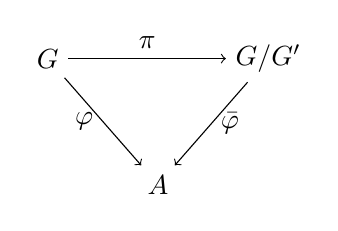
\begin{tikzpicture}[scale=1.0]
\node (G) at (0,1.6) {$G$};
\node (Q) at (2.8,1.6) {$G/G'$};
\node (A) at (1.4,0) {$A$};
\draw[->] (G)--node[above]{$\pi$}(Q);
\draw[->] (G)--node[left]{$\varphi$}(A);
\draw[->] (Q)--node[right]{$\bar{\varphi}$}(A);
\end{tikzpicture}
\end{center}
\end{enumerate}
\end{proposition}

\begin{proof}
（1）这由 \([x, y]\) 的定义立即得到。

（2）按定义，\(H \trianglelefteq G\) 当且仅当对所有 \(g \in G\) 和所有 \(h \in H\) 有 \(g^{-1}hg \in H\). 对 \(h \in H\)，\(g^{-1}hg \in H\) 当且仅当 \(h^{-1}g^{-1}hg \in H\)，故 \(H \trianglelefteq G\) 当且仅当对所有 \(h \in H\)、\(g \in G\) 有 \([h, g] \in H\). 于是 \(H \trianglelefteq G\) 当且仅当 \([H, G] \leq H\)，即（2）。

（3）设 \(\sigma \in \operatorname{Aut}(G)\)，\(x, y \in G\). 则
\[
\sigma([x, y]) = \sigma(x^{-1}y^{-1}xy) = \sigma(x)^{-1}\sigma(y)^{-1}\sigma(x)\sigma(y) = [\sigma(x), \sigma(y)].
\]
于是对 \(G'\) 的每个交换子 \([x, y]\)，\(\sigma([x, y])\) 仍是交换子。由于 \(\sigma\) 有双边逆，它把交换子集合双射到自身。由于交换子是 \(G'\) 的生成元集合，\(\sigma(G') = G'\)，即 \(G'\ \mathrm{char}\ G\).

为看出 \(G/G'\) 阿贝尔，设 \(xG'\)、\(yG'\) 是 \(G/G'\) 的任意元素。由 \(G/G'\) 中群运算的定义且 \([x, y] \in G'\)，我们有
\[
(xG')(yG') = (xy)G' = (yx[x, y])G' = (yx)G' = (yG')(xG'),
\]
完成（3）的证明。

（4）假设 \(H \trianglelefteq G\) 且 \(G/H\) 阿贝尔。则对所有 \(x, y \in G\) 有 \((xH)(yH) = (yH)(xH)\)，故
\[
1H = (xH)^{-1}(yH)^{-1}(xH)(yH) = x^{-1}y^{-1}xyH = [x, y]H.
\]
于是对所有 \(x, y \in G\) 有 \([x, y] \in H\)，故 \(G' \leq H\).

反之，若 \(G' \leq H\)，则由（3）\(G/G'\) 阿贝尔，故 \(G/G'\) 的每个子群都正规。特别地，\(H/G' \trianglelefteq G/G'\). 由格子同构定理，\(H \trianglelefteq G\). 由第三同构定理
\[
G/H \cong (G/G')/(H/G'),
\]
故 \(G/H\) 是阿贝尔群（同构于阿贝尔群 \(G/G'\) 的商）。这证明了（4）。

（5）这是用同态表述的（4）。
\end{proof}

取 \(G\) 对交换子子群的商把所有交换子坍缩为单位元，从而商群中所有元素都交换。正如（4）所示，其强逆命题也成立：\(G\) 对 \(H\) 的商是阿贝尔群当且仅当交换子子群包含在 \(H\) 中（即当且仅当 \(G'\) 在商 \(G/H\) 中映为单位元）。

我们将在下一节给出一个（96 阶的）群，它具有如下性质：其交换子子群中有一个元素不能写成任何 \(x, y\) 的单个交换子 \([x, y]\). 因此 \(G'\) 不一定仅由（单个）交换子的集合组成（而是由这些元素生成的群）。

\begin{example}
（1）群 \(G\) 是阿贝尔群当且仅当 \(G' = 1\).

（2）有时可以不具体计算交换子就求出群的交换子子群。例如，若 \(G = D_8\)，则由于 \(Z(D_8) = \langle r^2 \rangle \trianglelefteq D_8\) 且 \(D_8/Z(D_8)\) 是阿贝尔群（克莱因四元群），交换子子群 \(D_8'\) 是 \(Z(D_8)\) 的子群。由于 \(D_8\) 本身不阿贝尔，其交换子子群非平凡。唯一可能是 \(D_8' = Z(D_8)\). 由类似的论证，\(Q_8' = Z(Q_8) = \langle -1 \rangle\). 更一般地，若 \(G\) 是 \(p^3\) 阶（\(p\) 为素数）非阿贝尔群，则 \(G' = Z(G)\) 且 \(|G'| = p\)（习题 7）。

（3）设 \(D_{2n} = \langle r, s \mid r^n = s^2 = 1,\ s^{-1}rs = r^{-1} \rangle\). 由于 \([r, s] = r^{-2}\)，我们有 \(\langle r^{-2} \rangle = \langle r^2 \rangle \trianglelefteq D_{2n}\). 此外，\(\langle r^2 \rangle \trianglelefteq D_{2n}\)，且 \(r\) 与 \(s\) 在 \(D_{2n}/\langle r^2 \rangle\) 中的像生成这个商。它们是阶不超过 2 的交换元素，故商阿贝尔，且 \(D_{2n}' \leq \langle r^2 \rangle\). 于是 \(D_{2n}' = \langle r^2 \rangle\). 最后注意，若 \(n\)（\(= |r|\)）是奇数，则 \(\langle r^2 \rangle = \langle r \rangle\)；若 \(n\) 是偶数，则 \(\langle r^2 \rangle\) 在 \(\langle r \rangle\) 中指数为 2. 因此 \(D_{2n}'\) 在 \(D_{2n}\) 中的指数分别为 2 或 4，取决于 \(n\) 是奇数还是偶数。

（4）由于被 \(g \in G\) 共轭是 \(G\) 的自同构，由命题（3）对所有 \(a, b \in G\) 有 \([a^g, b^g] = [a, b]^g\)，即交换子的共轭也是交换子。例如，一旦我们把 \(S_n\) 中某个循环型的一个元素表示为交换子，那么同一循环型的所有元素也都是交换子（参见 4.3 节）。例如，每个 5-循环都是 \(S_5\) 中的交换子，理由如下：把五边形的顶点标为 \(1, \ldots, 5\)，我们看到 \(D_{10} \leq S_5\)（事实上是 \(A_5\) 的子群）。由前一个例子，5 阶元素是 \(D_{10}\) 中的交换子，从而是 \(S_5\) 中的交换子。具体地，
\[
(1\,4\,2\,5\,3) = [(1\,2\,3\,4\,5),\ (2\,5)(4\,3)].
\]
\end{example}

下一个结果实际上由命题 \ref{pro:3.13} 的证明推出，但我们把它单独列出以便引用：

\begin{proposition}\label{pro:5.8}
设 \(H\) 和 \(K\) 是群 \(G\) 的子群。集合 \(HK\) 中每个元素写成 \(hk\)（\(h \in H\)，\(k \in K\)）的不同方式的个数为 \(|H \cap K|\). 特别地，若 \(H \cap K = 1\)，则 \(HK\) 的每个元素都可以唯一地写成乘积 \(hk\)（\(h \in H\)，\(k \in K\)）。
\end{proposition}

\begin{proof}
留作练习。
\end{proof}

本节的主要结果是下面的识别定理。

\begin{theorem}\label{thm:5.9}
设 \(G\) 是群，\(H\) 和 \(K\) 是 \(G\) 的子群，满足

（1）\(H\) 和 \(K\) 在 \(G\) 中正规，且

（2）\(H \cap K = 1\).

则 \(HK \cong H \times K\).
\end{theorem}

\begin{proof}
注意由假设（1），\(HK\) 是 \(G\) 的子群（见推论 \ref{cor:3.15}）。设 \(h \in H\)、\(k \in K\). 由于 \(H \trianglelefteq G\)，\(k^{-1}hk \in H\)，故 \(h^{-1}(k^{-1}hk) \in H\). 类似地，\((h^{-1}k^{-1}h)k \in K\). 由于 \(H \cap K = 1\)，可知 \(h^{-1}k^{-1}hk = 1\)，即 \(hk = kh\)，所以 \(H\) 的每个元素与 \(K\) 的每个元素交换。

由前一个命题，\(HK\) 的每个元素可以唯一地写成乘积 \(hk\)（\(h \in H\)，\(k \in K\)）。因此映射
\[
\varphi : HK \to H \times K, \quad hk \mapsto (h, k)
\]
良定义。为看出 \(\varphi\) 是同态，注意若 \(h_1, h_2 \in H\)、\(k_1, k_2 \in K\)，则我们已经看到 \(h_2\) 与 \(k_1\) 交换。于是
\[
(h_1k_1)(h_2k_2) = (h_1h_2)(k_1k_2),
\]
而后一个乘积是把 \((h_1k_1)(h_2k_2)\) 写成 \(hk\)（\(h \in H\)，\(k \in K\)）的唯一方式。这表明
\[
\varphi(h_1k_1h_2k_2) = \varphi(h_1h_2k_1k_2) = (h_1h_2,\ k_1k_2) = (h_1, k_1)(h_2, k_2) = \varphi(h_1k_1)\varphi(h_2k_2),
\]
故 \(\varphi\) 是同态。同态 \(\varphi\) 是双射，因为 \(HK\) 的每个元素表示为 \(hk\) 形式的方式唯一，这证明 \(\varphi\) 是同构。
\end{proof}

\begin{definition}
若 \(G\) 是群，\(H\) 和 \(K\) 是 \(G\) 的满足 \(H \cap K = 1\) 的正规子群，则称 \(HK\) 为 \(H\) 和 \(K\) 的\textbf{内直积}。我们（在需要强调时）称 \(H \times K\) 为 \(H\) 和 \(K\) 的\textbf{外直积}。
\end{definition}

内直积与外直积的区别（由定理 \ref{thm:5.9}）纯粹是记号上的：内直积的元素写成 \(hk\) 的形式，而外直积的元素写成有序对 \((h, k)\). 我们在前面已经在这两者之间来回转换过。例如，当 \(Z_n = \langle a \rangle\)、\(Z_m = \langle b \rangle\) 时，我们写 \(x = (a, 1)\)、\(y = (1, b)\)，从而把 \(Z_n \times Z_m\) 的每个元素写成 \(x^r y^s\) 的形式。

\begin{example}
（1）若 \(n\) 是正奇数，我们证明 \(D_{4n} \cong D_{2n} \times Z_2\). 为看出这一点，设
\[
D_{4n} = \langle r, s \mid r^{2n} = s^2 = 1,\ srs = r^{-1} \rangle
\]
是 \(D_{4n}\) 的通常表示。设 \(H = \langle s, r^2 \rangle\)、\(K = \langle r^n \rangle\). 几何上，若 \(D_{4n}\) 是正 \(2n\) 边形的对称群，则 \(H\) 是把顶点 \(2i\) 与顶点 \(2i+2\)（对模 \(2n\) 的所有 \(i\)）连接起来所内接的正 \(n\) 边形的对称群（若令 \(\eta = r^2\)，则 \(H\) 有 \(2n\) 阶二面体群的通常表示，生成元为 \(\eta\) 和 \(s\)）。注意 \(H \trianglelefteq D_{4n}\)（指数为 2）。由于 \(|r| = 2n\)，有 \(|r^n| = 2\). 由于 \(srs = r^{-1}\)，有 \(sr^ns = r^{-n} = r^n\)，即 \(s\) 中心化 \(r^n\). 由于显然 \(r\) 中心化 \(r^n\)，有 \(K \leq Z(D_{4n})\). 故 \(K \trianglelefteq D_{4n}\). 最后，\(K \not\leq H\)，因为 \(r^2\) 有奇数阶（或者因为 \(r^n\) 把顶点 \(i\) 送到顶点 \(i+n\)，因而不保持 \(2n\) 边形的偶数顶点集）。于是由拉格朗日定理 \(H \cap K = 1\). 定理 \ref{thm:5.9} 于是完成证明。

（2）设 \(I\) 是 \(\{1, 2, \ldots, n\}\) 的子集，\(G\) 是 \(S_n\) 中 \(I\) 的集合稳定子，即
\[
G = \{\sigma \in S_n \mid \text{对所有 } i \in I \text{ 有 } \sigma(i) \in I\}.
\]
设 \(J = \{1, 2, \ldots, n\} - I\) 是 \(I\) 的补集，注意 \(G\) 也是 \(J\) 的集合稳定子。设 \(H\) 是 \(I\) 的点稳定子，\(K\) 是 \(\{1, 2, \ldots, n\} - I\) 的点稳定子，即
\[
H = \{\sigma \in G \mid \text{对所有 } i \in I \text{ 有 } \sigma(i) = i\}, \quad K = \{\tau \in G \mid \text{对所有 } j \in J \text{ 有 } \tau(j) = j\}.
\]
容易看出 \(H\) 和 \(K\) 是 \(G\) 的正规子群（事实上它们分别是 \(G\) 在 \(I\) 和 \(J\) 上作用的核）。由于 \(H \cap K\) 的任何元素固定 \(\{1, 2, \ldots, n\}\) 的所有元素，有 \(H \cap K = 1\). 最后，由于 \(G\) 的每个元素 \(\sigma\) 稳定集合 \(I\) 和 \(J\)，\(\sigma\) 的循环分解中每个循环只涉及 \(I\) 的元素或只涉及 \(J\) 的元素。于是 \(\sigma\) 可以写成乘积 \(\sigma_1\sigma_2\)，其中 \(\sigma_1 \in H\)、\(\sigma_2 \in K\). 这证明 \(G = HK\). 由定理 \ref{thm:5.9}，\(G \cong H \times K\). 现在 \(J\) 的任意置换可以通过令它在 \(I\) 上作为恒等映射而延拓为 \(S_n\) 中的置换。这些正是 \(H\) 中的置换（类似地，\(K\) 中的置换是在 \(J\) 上为恒等的 \(I\) 的置换），故
\[
H \cong S_{|J|}, \quad K \cong S_{|I|}, \quad \text{且} \quad G \cong S_m \times S_{n-m},
\]
其中 \(m = |I|\)（并约定 \(S_0 = 1\)）。

（3）设 \(\sigma \in S_n\)，\(I\) 是被 \(\sigma\) 逐点固定的 \(\{1, 2, \ldots, n\}\) 的子集：
\[
I = \{i \in \{1, 2, \ldots, n\} \mid \sigma(i) = i\}.
\]
若 \(C = C_{S_n}(\sigma)\)，则由第 4.3 节习题 18，\(C\) 稳定集合 \(I\) 及其补集 \(J\). 由前一个例子，\(C\) 同构于 \(H \times K\) 的一个子群，其中 \(H\) 是 \(S_n\) 中所有逐点固定 \(I\) 的置换构成的子群，\(K\) 是所有逐点固定 \(J\) 的置换的集合。注意 \(\sigma \in H\). 于是 \(C\) 的每个元素 \(\alpha\) 可以（唯一地）写成 \(\alpha = \alpha_1\alpha_2\)，其中 \(\alpha_1 \in H\)、\(\alpha_2 \in K\). 进一步注意，若 \(\tau\) 是 \(\{1, 2, \ldots, n\}\) 的任意固定每个 \(j \in J\) 的置换（即 \(K\) 的任意元素），则 \(\sigma\) 与 \(\tau\) 交换（因为它们不移动公共的整数）。于是 \(C\) 包含所有这样的 \(\tau\)，即 \(C\) 包含子群 \(K\). 这证明群 \(C\) 由所有这样的元素 \(\alpha_1\alpha_2 \in H \times K\) 组成：\(\alpha_2 \in K\) 任意，而 \(\alpha_1\) 在 \(H\) 中与 \(\sigma\) 交换：
\[
C_{S_n}(\sigma) = C_H(\sigma) \times K \cong C_{S_m}(\sigma) \times S_{n-m}.
\]
特别地，若 \(\sigma\) 是 \(S_n\) 中的 \(m\)-循环，则
\[
C_{S_n}(\sigma) = \langle \sigma \rangle \times S_{n-m}.
\]
后一个群的阶为 \(m(n-m)!\)，与 4.3 节算出的相同。
\end{example}

\subsection*{习题}
设 \(G\) 是群。

\begin{enumerate}
\item 证明：若 \(x, y \in G\)，则 \([y, x] = [x, y]^{-1}\). 由此推出对 \(G\) 的任意子集 \(A, B\) 有 \([A, B] = [B, A]\)（回忆 \([A, B]\) 是由交换子 \([a, b]\) 生成的 \(G\) 的子群）。

\item 证明 \(G\) 的子群 \(H\) 正规当且仅当 \([G, H] \leq H\).

\item 设 \(a, b, c \in G\). 证明

（a）\([a, bc] = [a, c](c^{-1}[a, b]c)\)；

（b）\([ab, c] = (b^{-1}[a, c]b)[b, c]\).

\item 求 \(S_4\) 和 \(A_4\) 的交换子子群。

\item 证明对所有 \(n \geq 5\)，\(A_n\) 是 \(S_n\) 的交换子子群。

\item 把 \(A_5\) 的每个循环型的一个代表在 \(S_5\) 中表示为交换子。

\item 证明：若 \(p\) 是素数，\(P\) 是 \(p^3\) 阶非阿贝尔群，则 \(P' = Z(P)\).

\item 假设 \(x, y \in G\) 且 \(x, y\) 都与 \([x, y]\) 交换。证明对所有 \(n \in \mathbb{Z}^+\)，
\[
(xy)^n = x^n y^n [y, x]^{\frac{n(n-1)}{2}}.
\]

\item 证明：若 \(p\) 是奇素数，\(P\) 是 \(p^3\) 阶群，则 \(p\) 次幂映射 \(x \mapsto x^p\) 是 \(P\) 到 \(Z(P)\) 的同态。若 \(P\) 不循环，证明 \(p\) 次幂映射的核的阶为 \(p^2\) 或 \(p^3\). 平方映射在 8 阶非阿贝尔群中是否同态？上述证明中哪里用到了 \(p\) 是奇数？〔使用习题 8。〕

\item 证明有限阿贝尔群是它的西罗子群的直积。

\item 证明：若 \(G = H \times K\)，其中 \(H\) 和 \(K\) 是 \(G\) 的特征子群且 \(H \cap K = 1\)，则 \(\operatorname{Aut}(G) \cong \operatorname{Aut}(H) \times \operatorname{Aut}(K)\). 由此推出：若 \(G\) 是有限阶阿贝尔群，则 \(\operatorname{Aut}(G)\) 同构于其西罗子群的自同构群的直积。

\item 用命题 \ref{pro:4.17} 描述有限循环群的自同构群。

\item 证明 \(D_{8n}\) 不同构于 \(D_{4n} \times Z_2\).

\item 设 \(G = \{(a_{ij}) \in GL_n(F) \mid a_{ij} = 0 \text{ 若 } i > j,\ \text{且 } a_{11} = a_{22} = \cdots = a_{nn}\}\)（\(F\) 是域）是对角元都相等的上三角矩阵构成的群。证明 \(G \cong D \times U\)，其中 \(D\) 是单位矩阵的所有非零倍数构成的群，\(U\) 是对角线上全为 1 的上三角矩阵构成的群。

\item 若 \(A\) 和 \(B\) 是 \(G\) 的正规子群且 \(G/A\) 和 \(G/B\) 都阿贝尔，证明 \(G/(A \cap B)\) 阿贝尔。

\item 证明：若 \(K\) 是 \(G\) 的正规子群，则 \(K' \trianglelefteq G\).

\item 若 \(K\) 是 \(G\) 的正规子群且 \(K\) 循环，证明 \(G' \leq C_G(K)\).〔回忆循环群的自同构群是阿贝尔群。〕

\item 设 \(K_1, K_2, \ldots, K_n\) 是非阿贝尔单群，\(G = K_1 \times K_2 \times \cdots \times K_n\). 证明 \(G\) 的每个正规子群都形如 \(\prod_{i \in I} K_i\)，其中 \(I\) 是 \(\{1, 2, \ldots, n\}\) 的某个子集（其中 \(\prod_{i \in \varnothing} K_i\) 定义为 1）。〔若 \(N \trianglelefteq G\) 不包含某个 \(K_i\)，取 \((a_1, \ldots, a_n) \in N\) 且 \(a_i \neq 1\)。证明 \([(1, \ldots, g_i, \ldots, 1), x] \in K_i \cap N\) 并推出 \(K_i \leq N\)。〕

\item 群 \(H\) 称为\textbf{完满的}，若 \(H' = H\)（即 \(H\) 等于它自己的交换子子群）。

（a）证明每个非阿贝尔单群都是完满的。

（b）证明：若 \(H\) 和 \(K\) 是群 \(G\) 的完满子群，则 \(\langle H, K \rangle\) 也完满。把它推广到 \(G\) 的任意一族完满子群生成的子群都完满。

（c）证明完满子群的任意共轭都完满。

（d）证明任何群 \(G\) 都有唯一的极大完满子群，且这个子群正规。

\item 设 \(H(F)\) 是域 \(F\) 上的海森伯群，参见第 1.4 节习题 11. 求交换子 \([X, Y]\)（\(X, Y \in H(F)\)）的具体公式，并证明 \(H(F)\) 的交换子子群等于 \(H(F)\) 的中心（参见第 2.2 节习题 14）。
\end{enumerate}

\section{半直积}

本节我们研究两个群 \(H\) 和 \(K\) 的“半直积”，它是 \(H\) 与 \(K\) 的直积概念的推广，做法是放宽 \(H\) 和 \(K\) 都正规这一要求。这个构造（在某些情形下）使我们能从群 \(H\) 和 \(K\) 构造一个“较大”的群 \(G\)，使 \(G\) 分别包含同构于 \(H\) 和 \(K\) 的子群，如直积的情形一样。此时子群 \(H\) 在 \(G\) 中正规，但子群 \(K\) 不一定正规（而在直积中是正规的）。因此，例如即使 \(H\) 和 \(K\) 阿贝尔，我们也能构造非阿贝尔群。这个构造将使我们能大大扩充可用的群的例子。与上一节一样，我们将接着证明一个识别定理，使我们能把一些熟悉的群分解为较小的“因子”，由此可以得到一些分类定理。

为引出动机，假设我们已经有一个群 \(G\) 包含子群 \(H\) 和 \(K\)，满足

（a）\(H \trianglelefteq G\)（但 \(K\) 不必在 \(G\) 中正规），且

（b）\(H \cap K = 1\).

\(HK\) 仍然是 \(G\) 的子群（推论 \ref{cor:3.15}），且由命题 \ref{pro:5.8}，\(HK\) 的每个元素都可以唯一地写成乘积 \(hk\)（\(h \in H\)，\(k \in K\)），即 \(HK\) 与有序对 \((h, k)\) 的集合之间存在双射，由 \(hk \mapsto (h, k)\) 给出（从而群 \(H\) 表现为元素 \((h, 1)\) 的集合，\(K\) 表现为元素 \((1, k)\) 的集合）。给定 \(HK\) 的两个元素 \(h_1k_1\) 和 \(h_2k_2\)，我们首先看如何把它们的乘积（在 \(G\) 中）写成同样的形式：
\[
\begin{aligned}
(h_1k_1)(h_2k_2) &= h_1k_1h_2(k_1^{-1}k_1)k_2 \\
&= h_1(k_1h_2k_1^{-1})k_1k_2 \\
&= h_3k_3,
\end{aligned} \tag{5.1}
\]
其中 \(h_3 = h_1(k_1h_2k_1^{-1})\)、\(k_3 = k_1k_2\). 注意由于 \(H \trianglelefteq G\)，\(k_1h_2k_1^{-1} \in H\)，故 \(h_3 \in H\)、\(k_3 \in K\).

这些计算的前提是已经存在一个群 \(G\) 包含满足 \(H \trianglelefteq G\)、\(H \cap K = 1\) 的子群 \(H\) 和 \(K\)。半直积的基本想法是把这一构造反过来，即从两个（抽象）群 \(H\) 和 \(K\) 出发，试图定义一个包含它们（的同构复制）的群，使上面（a）和（b）成立。为此，我们把定义群中元素乘法的等式 (1) 写成一种在我们尚不知道是否存在上述群 \(G\) 时也有意义的形式。关键在于：(1) 中的 \(k_3\) 只由 \(K\) 中的乘法（即 \(k_1k_2\)）得到，而 \(h_3\) 由把 \(h_1\) 与 \(k_1h_2k_1^{-1}\) 在 \(H\) 中相乘得到。如果我们能理解元素 \(k_1h_2k_1^{-1}\) 从何而来（用 \(H\) 和 \(K\) 表示，而不涉及 \(G\)），那么群 \(HK\) 就完全用 \(H\) 和 \(K\) 描述出来了。然后我们可以用这个描述，用等式 (1) 来定义乘法，从而定义群 \(HK\).

由于 \(H\) 在 \(G\) 中正规，群 \(K\) 通过共轭作用在 \(H\) 上：
\[
k \cdot h = khk^{-1} \quad \text{对 } h \in H,\ k \in K
\]
（我们用符号 \(\cdot\) 强调这是一个作用），于是 (1) 可以写成
\[
(h_1k_1)(h_2k_2) = (h_1\, k_1 \cdot h_2)(k_1k_2). \tag{5.2}
\]
\(K\) 通过共轭在 \(H\) 上的作用给出 \(K\) 到 \(\operatorname{Aut}(H)\) 的一个同态 \(\varphi\)，所以 (2) 表明 \(HK\) 中的乘法只依赖于 \(H\) 中的乘法、\(K\) 中的乘法以及同态 \(\varphi\)，因此完全用 \(H\) 和 \(K\) 内蕴地定义。

现在用这个解释，从两个群 \(H\) 和 \(K\) 以及一个同态 \(\varphi : K \to \operatorname{Aut}(H)\) 出发来定义一个群（它将被证明定义了所得到的群中的共轭）。

\begin{theorem}\label{thm:5.10}
设 \(H\) 和 \(K\) 是群，\(\varphi\) 是从 \(K\) 到 \(\operatorname{Aut}(H)\) 的同态。用 \(\cdot\) 表示由 \(\varphi\) 确定的 \(K\) 在 \(H\) 上的（左）作用。设 \(G\) 是满足 \(h \in H\)、\(k \in K\) 的有序对 \((h, k)\) 的集合，并在 \(G\) 上定义如下乘法：
\[
(h_1, k_1)(h_2, k_2) = (h_1\, k_1 \cdot h_2,\ k_1k_2).
\]
则

（1）这个乘法使 \(G\) 成为阶为 \(|G| = |H||K|\) 的群。

（2）集合 \(\{(h, 1) \mid h \in H\}\) 和 \(\{(1, k) \mid k \in K\}\) 是 \(G\) 的子群，且映射 \(h \mapsto (h, 1)\)（\(h \in H\)）和 \(k \mapsto (1, k)\)（\(k \in K\)）分别是这些子群与群 \(H\) 和 \(K\) 的同构：
\[
H \cong \{(h, 1) \mid h \in H\}, \quad K \cong \{(1, k) \mid k \in K\}.
\]

把 \(H\) 和 \(K\) 与（2）中所述的它们在 \(G\) 中的同构复制等同，我们有

（3）\(H \trianglelefteq G\)；

（4）\(H \cap K = 1\)；

（5）对所有 \(h \in H\)、\(k \in K\) 有 \(khk^{-1} = k \cdot h = \varphi(k)(h)\).
\end{theorem}

\begin{proof}
利用 \(\cdot\) 是 \(K\) 在 \(H\) 上的作用这一事实，容易验证 \(G\) 在这个乘法下是群。例如，结合律验证如下：对所有 \((a, x), (b, y), (c, z) \in G\)，
\[
\begin{aligned}
((a, x)(b, y))(c, z) &= (a\, x \cdot b,\ xy)(c, z) \\
&= (a\, x \cdot b\, (xy) \cdot c,\ xyz) \\
&= (a\, x \cdot b\, x \cdot (y \cdot c),\ xyz) \\
&= (a\, x \cdot (b\, y \cdot c),\ xyz) \\
&= (a, x)(b\, y \cdot c,\ yz) = (a, x)((b, y)(c, z)).
\end{aligned}
\]
我们把验证 \((1, 1)\) 是 \(G\) 的单位元、以及
\[
(h, k)^{-1} = (k^{-1} \cdot h^{-1},\ k^{-1})
\]
对每个 \((h, k) \in G\) 成立留作练习。群 \(G\) 的阶显然是 \(H\) 与 \(K\) 的阶之积，这证明了（1）。

设 \(\bar{H} = \{(h, 1) \mid h \in H\}\)、\(\bar{K} = \{(1, k) \mid k \in K\}\). 对所有 \(a, b \in H\) 有
\[
(a, 1)(b, 1) = (a\, 1 \cdot b,\ 1) = (ab, 1),
\]
且对所有 \(x, y \in K\) 有
\[
(1, x)(1, y) = (1, xy),
\]
这表明 \(\bar{H}\) 和 \(\bar{K}\) 是 \(G\) 的子群，且（2）中的映射是同构。

显然 \(\bar{H} \cap \bar{K} = 1\)，即（4）。现在，
\[
\begin{aligned}
(1, k)(h, 1)(1, k)^{-1} &= ((1, k)(h, 1))(1, k^{-1}) \\
&= (k \cdot h,\ k)(1, k^{-1}) \\
&= (k \cdot h\, k \cdot 1,\ kk^{-1}) \\
&= (k \cdot h,\ 1),
\end{aligned}
\]
故由（2）中把 \((h, 1)\) 与 \(h\) 等同、\((1, k)\) 与 \(k\) 等同，我们有 \(khk^{-1} = k \cdot h\)，即（5）。

最后，我们刚刚看到（在（2）的等同下）\(K \leq N_G(H)\). 由于 \(G = HK\) 且当然 \(H \leq N_G(H)\)，我们有 \(N_G(H) = G\)，即 \(H \trianglelefteq G\)，这证明了（3）并完成证明。
\end{proof}

\begin{definition}
设 \(H\) 和 \(K\) 是群，\(\varphi\) 是从 \(K\) 到 \(\operatorname{Aut}(H)\) 的同态。定理 \ref{thm:5.10} 中描述的群称为 \(H\) 和 \(K\) 关于 \(\varphi\) 的\textbf{半直积}，记作 \(H \rtimes_\varphi K\)（若无混淆之虞，我们简写为 \(H \rtimes K\)）。
\end{definition}

这个记号的选择是为了提醒我们 \(H\) 在 \(H \rtimes K\) 中的复制是正规的“因子”，且半直积的构造对 \(H\) 和 \(K\) 不是对称的（不像直积）。在给出一些例子之前，我们弄清半直积何时就是直积（特别地，我们看到直积是半直积的特例）。另见习题 1。

\begin{proposition}\label{pro:5.11}
设 \(H\) 和 \(K\) 是群，\(\varphi : K \to \operatorname{Aut}(H)\) 是同态。则下列命题等价：

（1）\(H \rtimes_\varphi K\) 与 \(H \times K\) 之间的恒等（集合）映射是群同态（从而是同构）；

（2）\(\varphi\) 是从 \(K\) 到 \(\operatorname{Aut}(H)\) 的平凡同态；

（3）\(K \trianglelefteq H \rtimes_\varphi K\).
\end{proposition}

\begin{proof}
（1）\(\Rightarrow\)（2）：由 \(H \rtimes K\) 中群运算的定义，
\[
(h_1, k_1)(h_2, k_2) = (h_1\, k_1 \cdot h_2,\ k_1k_2)
\]
对所有 \(h_1, h_2 \in H\)、\(k_1, k_2 \in K\) 成立。由假设（1），\((h_1, k_1)(h_2, k_2) = (h_1h_2, k_1k_2)\). 比较这些有序对的第一个分量得 \(k_1 \cdot h_2 = h_2\) 对所有 \(h_2 \in H\) 和所有 \(k_1 \in K\) 成立，即 \(K\) 平凡地作用在 \(H\) 上。这就是（2）。

（2）\(\Rightarrow\)（3）：若 \(\varphi\) 平凡，则 \(K\) 在 \(H\) 上的作用平凡，故由定理 \ref{thm:5.10}(5)，\(H\) 的元素与 \(K\) 的元素交换。特别地，\(H\) 正规化 \(K\). 由于 \(K\) 正规化自身，\(G = HK\) 正规化 \(K\)，即（3）。

（3）\(\Rightarrow\)（1）：若 \(K\) 在 \(H \rtimes K\) 中正规，则（如同定理 \ref{thm:5.9} 的证明）对所有 \(h \in H\)、\(k \in K\) 有 \([h, k] \in H \cap K = 1\). 故 \(hk = kh\)，\(K\) 在 \(H\) 上的作用平凡。于是半直积中的乘法与直积中的相同：
\[
(h_1, k_1)(h_2, k_2) = (h_1h_2, k_1k_2)
\]
对所有 \(h_1, h_2 \in H\)、\(k_1, k_2 \in K\) 成立。这给出（1）并完成证明。
\end{proof}

\begin{example}
在所有例子中 \(H\) 和 \(K\) 是群，\(\varphi\) 是从 \(K\) 到 \(\operatorname{Aut}(H)\) 的同态，与它相伴的 \(K\) 在 \(H\) 上的作用用点号表示。设 \(G = H \rtimes K\)，并如定理 \ref{thm:5.10} 那样把 \(H\) 和 \(K\) 与 \(G\) 的子群等同。我们将用命题 \ref{pro:4.16} 和 \ref{pro:4.17} 对某些具体的群 \(H\) 确定同态 \(\varphi\). 在下面每个例子中，证明 \(\varphi\) 是同态都很容易（因为 \(K\) 往往是循环群），故省略细节。

（1）设 \(H\) 是任意阿贝尔群（甚至无限阶的），\(K = \langle x \rangle \cong Z_2\) 是 2 阶群。定义 \(\varphi : K \to \operatorname{Aut}(H)\) 为把 \(x\) 映到 \(H\) 上的取逆自同构，于是相应的作用是 \(x \cdot h = h^{-1}\)（对所有 \(h \in H\)）。则 \(G\) 包含指数为 2 的子群 \(H\)，且
\[
xhx^{-1} = h^{-1} \quad \text{对所有 } h \in H.
\]
特别有趣的是 \(H\) 循环的情形：若 \(H = Z_n\)，则 \(G\) 就是 \(D_{2n}\)；若 \(H = \mathbb{Z}\)，我们把 \(G\) 记作 \(D_\infty\).

（2）我们可以用若干方式推广前一个例子。一种方式是让 \(H\) 是任意阿贝尔群，让 \(K = \langle x \rangle \cong Z_{2n}\) 是 \(2n\) 阶循环群。仍定义 \(\varphi\) 为把 \(x\) 映到取逆自同构，于是 \(x^2\) 在 \(H\) 上作为恒等映射。在 \(G\) 中，\(xhx^{-1} = h^{-1}\) 且 \(x^2hx^{-2} = h\) 对所有 \(h \in H\) 成立。故 \(x^2 \in Z(G)\). 特别地，若 \(H = Z_3\)、\(K = Z_4\)，则 \(G\) 是 12 阶非阿贝尔群，它不同构于 \(A_4\) 或 \(D_{12}\)（因为它的西罗 2-子群 \(K\) 是 4 阶循环群）。

（3）承接前一个例子，设 \(H = \langle h \rangle \cong Z_{2^n}\)、\(K = \langle x \rangle \cong Z_4\)，在 \(G\) 中 \(xhx^{-1} = h^{-1}\). 如上所述 \(x^2 \in Z(G)\). 由于 \(x\) 把 \(h\) 取逆（即把 \(H\) 取逆），\(x\) 把 \(H\) 中唯一的 2 阶子群 \(\langle z \rangle\) 取逆，其中 \(z = h^{2^{n-1}}\). 于是 \(xzx^{-1} = z^{-1} = z\)，故 \(x\) 中心化 \(z\). 由此推出 \(z \in Z(G)\). 于是 \(x^2z \in Z(G)\)，从而 \(\langle x^2z \rangle \trianglelefteq G\). 令 \(\bar{G} = G/\langle x^2z \rangle\). 由于 \(x^2\) 和 \(z\) 是不同的 2 阶交换元素，\(x^2z\) 的阶为 2，故 \(|\bar{G}| = \frac{1}{2}|G| = 2^{n+1}\). 通过取出乘积 \(x^2z\) 作商，我们把 \(x^2\) 与 \(h^{2^{n-1}}\) 在商中等同起来。特别地，当 \(n = 2\) 时，\(x\) 和 \(h\) 的阶都是 4，\(x\) 把 \(h\) 取逆且 \(\bar{G} = \langle x^2 \rangle\). 由此推出此时 \(\bar{G} \cong Q_8\). 一般地，可以验证 \(\bar{G}\) 有唯一的 2 阶子群（即 \(\langle x^2 \rangle\)），它等于 \(\bar{G}\) 的中心。群 \(\bar{G}\) 称为 \(2^{n+1}\) 阶\textbf{广义四元数群}，记作 \(Q_{2^{n+1}}\)：
\[
Q_{2^{n+1}} = \langle h, x \mid h^{2^n} = x^4 = 1,\ x^{-1}hx = h^{-1},\ h^{2^{n-1}} = x^2 \rangle.
\]

（4）设 \(H = \mathbb{Q}\)（加法下），\(K = \langle x \rangle \cong \mathbb{Z}\). 定义 \(\varphi\) 为把 \(x\) 映到 \(H\) 上的“乘以 2”映射，于是 \(x\) 通过 \(x \cdot h = 2h\) 作用在 \(h \in H\) 上。注意乘以 2 是 \(H\) 的自同构，因为它有双边逆，即乘以 \(\frac{1}{2}\). 在群 \(G\) 中，\(\mathbb{Z} \leq \mathbb{Q}\) 且 \(\mathbb{Z}\) 的共轭 \(x\mathbb{Z}x^{-1}\) 是 \(\mathbb{Z}\) 的真子群（即 \(2\mathbb{Z}\)）。因此 \(x\mathbb{Z}x^{-1} \neq \mathbb{Z}\)，尽管 \(x\mathbb{Z}x^{-1} \leq \mathbb{Z}\). 换言之，要证明元素 \(g\) 正规化无限群中的子群 \(A\)，一般不能只证明 \(A\) 被 \(g\) 共轭后包含在 \(A\) 中（这对有限群是充分的）。

（5）对任意群 \(H\)，设 \(K = \operatorname{Aut}(H)\)，\(\varphi\) 是从 \(K\) 到 \(\operatorname{Aut}(H)\) 的恒等同态。半直积 \(H \rtimes \operatorname{Aut}(H)\) 称为 \(H\) 的\textbf{全形}，记作 \(\operatorname{Hol}(H)\). 下面描述了一些全形；这些同构的验证作为本章末的习题给出。

（a）\(\operatorname{Hol}(Z_2 \times Z_2) \cong S_4\).

（b）若 \(|G| = n\) 且 \(\pi : G \to S_n\) 是左正则表示（4.2 节），则 \(N_{S_n}(\pi(G)) \cong \operatorname{Hol}(G)\). 特别地，由于 \(Z_n\) 的生成元的左正则表示是 \(S_n\) 中的 \(n\)-循环，我们对任意 \(n\)-循环 \((1\,2\,\ldots\,n)\) 得到
\[
N_{S_n}(\langle (1\,2\,\ldots\,n) \rangle) \cong \operatorname{Hol}(Z_n) = Z_n \rtimes \operatorname{Aut}(Z_n).
\]
注意后一个群的阶为 \(n\varphi(n)\).

（6）设 \(p\) 和 \(q\) 是素数且 \(p < q\)，\(H = Z_q\)、\(K = Z_p\). 我们已经看到若 \(p\) 不整除 \(q-1\)，则每个 \(pq\) 阶群都循环（见命题 \ref{pro:4.16} 后的例子）。这与以下事实一致：若 \(p\) 不整除 \(q-1\)，则不存在从 \(Z_p\) 到 \(\operatorname{Aut}(Z_q)\) 的非平凡同态（由命题 \ref{pro:4.17}，后者是 \(q-1\) 阶循环群）。现在假设 \(p \mid q-1\). 由柯西定理，\(\operatorname{Aut}(Z_q)\) 含有 \(p\) 阶子群（它唯一，因为 \(\operatorname{Aut}(Z_q)\) 循环）。于是存在从 \(K\) 到 \(\operatorname{Aut}(H)\) 的非平凡同态 \(\varphi\). 相应的群 \(G = H \rtimes_\varphi K\) 的阶为 \(pq\)，且 \(K\) 在 \(G\) 中不正规（命题 \ref{pro:5.11}）。特别地，\(G\) 非阿贝尔。我们不久将证明 \(G\) 是（在同构意义下）唯一的 \(pq\) 阶非阿贝尔群。若 \(p = 2\)，\(G\) 必同构于 \(D_{2q}\).

（7）设 \(p\) 是奇素数。我们构造两个 \(p^3\) 阶互不同构的非阿贝尔群（我们将证明任意 \(p^3\) 阶非阿贝尔群都同构于这两个之一）。

设 \(H = Z_p \times Z_p\)、\(K = Z_p\). 由命题 \ref{pro:4.17}，\(\operatorname{Aut}(H) \cong GL_2(\mathbb{F}_p)\) 且 \(|\operatorname{GL}_2(\mathbb{F}_p)| = (p^2-1)(p^2-p)\). 由于 \(p \mid |\operatorname{Aut}(H)|\)，由柯西定理 \(H\) 有 \(p\) 阶自同构。于是存在从 \(K\) 到 \(\operatorname{Aut}(H)\) 的非平凡同态 \(\varphi\)，故相应的群 \(H \rtimes_\varphi K\) 是 \(p^3\) 阶非阿贝尔群。更具体地说，若 \(H = \langle a \rangle \times \langle b \rangle\)、\(x\) 是 \(K\) 的生成元，则 \(x\) 通过
\[
x \cdot a = ab, \quad x \cdot b = b
\]
作用在 \(a\) 和 \(b\) 上，这定义了 \(x\) 在整个 \(H\) 上的作用。关于 \(H\) 作为 2 维向量空间的 \(\mathbb{F}_p\)-基 \(a, b\)，\(x\) 的作用（可以看作加法记号下的非奇异线性变换）有矩阵
\[
\begin{pmatrix} 1 & 1 \\ 0 & 1 \end{pmatrix} \in GL_2(\mathbb{F}_p).
\]
所得的半直积有表示
\[
\langle x, a, b \mid x^p = a^p = b^p = 1,\ ab = ba,\ xax^{-1} = ab,\ xbx^{-1} = b \rangle
\]
（事实上这个群由 \(\{x, a\}\) 生成，称为 \(\mathbb{Z}/p\mathbb{Z}\) 上的海森伯群，参见习题 25）。

接下来设 \(H = Z_{p^2}\)、\(K = Z_p\). 再由命题 \ref{pro:4.17}，\(\operatorname{Aut}(H) \cong Z_{p(p-1)}\)，故 \(H\) 有 \(p\) 阶自同构。于是存在从 \(K\) 到 \(\operatorname{Aut}(H)\) 的非平凡同态 \(\varphi\)，故群 \(H \rtimes_\varphi K\) 非阿贝尔且阶为 \(p^3\). 更具体地说，若 \(H = \langle y \rangle\)、\(x\) 是 \(K\) 的生成元，则 \(x\) 通过
\[
x \cdot y = y^{1+p}
\]
作用在 \(y\) 上。所得的半直积有表示
\[
\langle x, y \mid x^p = y^{p^2} = 1,\ xyx^{-1} = y^{1+p} \rangle.
\]
这两个群不同构（前者不含 \(p^2\) 阶元素，参见习题 25；后者显然含有，即 \(y\)）。

（8）设 \(H = Q_8 \times (Z_2 \times Z_2) = \langle i, j \rangle \times (\langle a \rangle \times \langle b \rangle)\)，\(K = \langle y \rangle \cong Z_3\). 由
\[
i \mapsto j,\quad j \mapsto k = ij,\quad a \mapsto b,\quad b \mapsto ab
\]
定义的映射容易看出给出 \(H\) 的一个 3 阶自同构。设 \(\varphi\) 是由把 \(y\) 映到这个自同构所定义的从 \(K\) 到 \(\operatorname{Aut}(H)\) 的同态，\(G\) 是相应的半直积，于是 \(y \in G\) 通过
\[
y \cdot i = j,\quad y \cdot j = k,\quad y \cdot a = b,\quad y \cdot b = ab
\]
作用。群 \(G = H \rtimes_\varphi K\) 是 96 阶非阿贝尔群，具有性质：元素 \(i^2a \in G'\)，但 \(i^2a\) 不能表示为任何 \(x, y \in G\) 的单个交换子 \([x, y]\)（验证后一断言是初等计算）。
\end{example}

与直积的情形一样，我们现在证明半直积的一个识别定理。这个定理将使我们能“分解”某些阶的群，从而分类这些阶的群。策略在定理之后详细讨论。

\begin{theorem}\label{thm:5.12}
设 \(G\) 是群，\(H\) 和 \(K\) 是 \(G\) 的子群，满足

（1）\(H \trianglelefteq G\)，且

（2）\(H \cap K = 1\).

设 \(\varphi : K \to \operatorname{Aut}(H)\) 是由把 \(k \in K\) 映到 \(k\) 在 \(H\) 上的左共轭自同构所定义的同态。则 \(HK \cong H \rtimes_\varphi K\). 特别地，若 \(G = HK\) 且 \(H\) 和 \(K\) 满足（1）和（2），则 \(G\) 是 \(H\) 和 \(K\) 的半直积。
\end{theorem}

\begin{proof}
注意由于 \(H \trianglelefteq G\)，\(HK\) 是 \(G\) 的子群。由命题 \ref{pro:5.8}，\(HK\) 的每个元素可以唯一地写成 \(hk\)（\(h \in H\)，\(k \in K\)）。因此映射 \(hk \mapsto (h, k)\) 是从 \(HK\) 到 \(H \rtimes K\) 的集合双射。这个映射是同态这一事实正是本节开始时把我们引向半直积定义的那个计算。
\end{proof}

\begin{definition}
设 \(H\) 是群 \(G\) 的子群。\(G\) 的子群 \(K\) 称为 \(H\) 在 \(G\) 中的\textbf{补}，若 \(G = HK\) 且 \(H \cap K = 1\).
\end{definition}

有了这个术语，识别半直积的准则就简单地说成：必须存在 \(G\) 的某个真正规子群的补。并非每个群都是它的两个真子群的半直积（例如单群），但如我们所见，半直积的概念大大扩充了我们已知的群的列表。

\subsection*{一些分类}

现在我们应用定理 \ref{thm:5.12} 对某些 \(n\) 值分类 \(n\) 阶群。下面每个论证的基本思想是

（a）证明每个 \(n\) 阶群都有真子群 \(H\) 和 \(K\)，满足定理 \ref{thm:5.12} 的假设且 \(G = HK\)；

（b）求出 \(H\) 和 \(K\) 的所有可能的同构类型；

（c）对（b）中求出的每一对 \(H, K\)，求出所有可能的同态 \(\varphi : K \to \operatorname{Aut}(H)\)；

（d）对（c）中求出的每个三元组 \(H, K, \varphi\)，构造半直积 \(H \rtimes_\varphi K\)（于是任何 \(n\) 阶群 \(G\) 都同构于这些具体构造的群之一），并在所有这些半直积中确定哪些对同构。这就得到 \(n\) 阶群的互不同构类型的列表。

为了开始这个过程，我们首先必须找到（任意 \(n\) 阶群 \(G\) 的）满足上述条件的子群 \(H\) 和 \(K\)。对“较小”的 \(n\)，我们常常可以用西罗定理做到这一点。为证明 \(H\) 正规，我们用西罗定理的共轭部分或第 4 章建立的其他正规性判别准则（例如推论 \ref{cor:4.5}）。其中一些工作已在 4.5 节的例子中完成。在下面许多例子中，\(|H|\) 与 \(|K|\) 互素，故由拉格朗日定理 \(H \cap K = 1\).

由于 \(H\) 和 \(K\) 是 \(G\) 的真子群，应当把 \(H\) 和 \(K\) 的确定看作归纳地完成的。在我们讨论的例子中，\(H\) 和 \(K\) 的阶足够小，以致我们由前面的结果知道它们所有可能的同构类型。例如，在大多数情形 \(H\) 和 \(K\) 的阶是素数或素数的平方。

在我们例子中，可能的同态 \(\varphi : K \to \operatorname{Aut}(H)\) 相对较少，特别在考虑到某些对称性之后（例如当 \(K\) 循环时把 \(K\) 的一个生成元换成另一个）。

最后，这个过程得到的半直积在我们的例子中数量很少，我们将发现它们大多（两两）不同构。一般地，这可能是一个更微妙的问题，如习题 4 所示。

我们强调，这种把某个给定阶 \(n\) 的每个群“分解”为半直积的做法对任意 \(n\) 不成立。例如 \(Q_8\) 不是半直积，因为没有任何真子群有补（尽管我们看到它是一个半直积的商）。经验上，当群阶 \(n\) 不被任何素数的大幂整除时，这个过程通常很有效。在另一个极端，对大 \(a\) 的 \(p^a\) 阶群（\(p\) 为素数）中，只有一小部分是非平凡半直积。

\begin{example}[\(pq\) 阶群，\(p, q\) 是素数且 \(p < q\)]
设 \(G\) 是任意 \(pq\) 阶群，\(P \in \operatorname{Syl}_p(G)\)、\(Q \in \operatorname{Syl}_q(G)\). 在西罗定理应用的第 1 个例子中我们证明了 \(G \cong Q \rtimes_\varphi P\)，对某个 \(\varphi : P \to \operatorname{Aut}(Q)\). 由于 \(P\) 和 \(Q\) 的阶是素数，它们循环。群 \(\operatorname{Aut}(Q)\) 是 \(q-1\) 阶循环群。若 \(p\) 不整除 \(q-1\)，则从 \(P\) 到 \(\operatorname{Aut}(Q)\) 的唯一同态是平凡同态，故此时唯一的半直积是直积，即 \(G\) 循环。

现在考虑 \(p \mid q-1\) 的情形，设 \(P = \langle y \rangle\). 由于 \(\operatorname{Aut}(Q)\) 循环，它含有唯一的 \(p\) 阶子群，设为 \(\langle \gamma \rangle\). 任何同态 \(\varphi : P \to \operatorname{Aut}(Q)\) 必把 \(y\) 映到 \(\gamma\) 的某个幂。因此有 \(p\) 个同态 \(\varphi_i : P \to \operatorname{Aut}(Q)\)，由 \(\varphi_i(y) = \gamma^i\)（\(0 \leq i \leq p-1\)）给出。由于 \(\varphi_0\) 是平凡同态，如前 \(Q \rtimes_{\varphi_0} P \cong Q \times P\). 每个 \(i \neq 0\) 的 \(\varphi_i\) 给出一个 \(pq\) 阶非阿贝尔群 \(G_i\). 容易验证这些群都同构，因为对每个 \(\varphi_i\)（\(i > 0\)），存在 \(P\) 的某个生成元 \(y_i\) 使 \(\varphi_i(y_i) = \gamma\). 因此，在选取 \(P\) 的（任意）生成元的意义下，这些半直积都相同（见习题 6，另见第 4.3 节习题 28）。
\end{example}

\begin{example}[30 阶群]
由西罗定理之后的例子，每个 30 阶群 \(G\) 都含有 15 阶子群 \(H\). 由前一个例子，\(H\) 循环且 \(H\) 在 \(G\) 中正规（指数为 2）。由西罗定理，\(G\) 有 2 阶子群 \(K\). 于是 \(G = HK\) 且 \(H \cap K = 1\)，故对某个 \(\varphi : K \to \operatorname{Aut}(H)\) 有 \(G \cong H \rtimes_\varphi K\). 由命题 \ref{pro:4.16}，
\[
\operatorname{Aut}(Z_{15}) \cong (\mathbb{Z}/15\mathbb{Z})^\times \cong Z_4 \times Z_2.
\]
后一个同构可以直接计算，也可以用上一节的习题 11：把 \(H\) 写成 \(\langle a \rangle \times \langle b \rangle \cong Z_5 \times Z_3\)，则（由于这两个子群在 \(H\) 中特征）
\[
\operatorname{Aut}(H) \cong \operatorname{Aut}(Z_5) \times \operatorname{Aut}(Z_3).
\]
特别地，\(\operatorname{Aut}(H)\) 恰含有三个 2 阶元素，它们在群 \(H = \langle a \rangle \times \langle b \rangle\) 上的作用如下：
\[
a \mapsto a,\ b \mapsto b^{-1}; \qquad a \mapsto a^{-1},\ b \mapsto b; \qquad a \mapsto a^{-1},\ b \mapsto b^{-1}.
\]
因此有三个从 \(K\) 到 \(\operatorname{Aut}(H)\) 的非平凡同态，由把 \(K\) 的生成元映到这三个 2 阶元素之一给出（照例，平凡同态给出直积：\(H \times K \cong Z_{30}\)）。

设 \(K = \langle k \rangle\). 若同态 \(\varphi_1 : K \to \operatorname{Aut}(H)\) 由把 \(k\) 映到上面第一个自同构所定义（于是 \(k \cdot a = a\)、\(k \cdot b = b^{-1}\) 给出 \(k\) 在 \(H\) 上的作用），则容易看出 \(G_1 = H \rtimes_{\varphi_1} K\) 同构于 \(Z_5 \times D_6\)（注意在这个半直积中 \(k\) 中心化 \(H\) 的 5 阶元素 \(a\)，故作为直积的分解为 \(\langle a \rangle \times \langle b, k \rangle\)）。

若 \(\varphi_2\) 由把 \(k\) 映到上面第二个自同构所定义，则容易看出 \(G_2 = H \rtimes_{\varphi_2} K\) 同构于 \(Z_3 \times D_{10}\)（注意在这个半直积中 \(k\) 中心化 \(H\) 的 3 阶元素 \(b\)，故作为直积的分解为 \(\langle b \rangle \times \langle a, k \rangle\)）。

若 \(\varphi_3\) 由把 \(k\) 映到上面第三个自同构所定义，则容易看出 \(G_3 = H \rtimes_{\varphi_3} K\) 同构于 \(D_{30}\).

注意这些群都不同构，因为它们的中心阶分别为 30（阿贝尔情形）、5（\(G_1\)）、3（\(G_2\)）和 1（\(G_3\)）。

我们强调，虽然（事后看来）这个过程没有给出任何我们不能仅用直积构造出的群，但这个论证证明了这是 30 阶群同构类型的完整列表。
\end{example}

\begin{example}[12 阶群]
设 \(G\) 是 12 阶群，\(V \in \operatorname{Syl}_2(G)\)、\(T \in \operatorname{Syl}_3(G)\). 由 4.5 节对 12 阶群的讨论我们知道 \(V\) 或 \(T\) 在 \(G\) 中正规（为作说明，我们不调用第 4 章结果的全力，即或者 \(T \trianglelefteq G\) 或者 \(G \cong A_4\)）。由拉格朗日定理 \(V \cap T = 1\). 因此 \(G\) 是半直积。注意 \(V \cong Z_4\) 或 \(Z_2 \times Z_2\)，且 \(T \cong Z_3\).

\textbf{情形 1：}\(V \trianglelefteq G\).

我们必须确定从 \(T\) 到 \(\operatorname{Aut}(V)\) 的所有可能同态。若 \(V \cong Z_4\)，则 \(\operatorname{Aut}(V) \cong Z_2\)，不存在从 \(T\) 到 \(\operatorname{Aut}(V)\) 的非平凡同态。因此有正规循环西罗 2-子群的唯一 12 阶群是 \(Z_{12}\).

因此假设 \(V \cong Z_2 \times Z_2\). 此时 \(\operatorname{Aut}(V) \cong S_3\)，且 \(\operatorname{Aut}(V)\) 有唯一的 3 阶子群，设为 \(\langle \gamma \rangle\). 于是若 \(T = \langle y \rangle\)，有三个从 \(T\) 到 \(\operatorname{Aut}(V)\) 的可能同态：
\[
\varphi_i : T \to \operatorname{Aut}(V), \quad \text{由 } \varphi_i(y) = \gamma^i \text{ 定义},\ i = 0, 1, 2.
\]
照例，\(\varphi_0\) 是平凡同态，给出直积 \(Z_2 \times Z_2 \times Z_3\). 同态 \(\varphi_1\) 和 \(\varphi_2\) 给出同构的半直积，因为它们只相差 \(T\) 的生成元的选取（即 \(\varphi_1(y) = \gamma\) 且 \(\varphi_2(y') = \gamma\)，其中 \(y' = y^2\) 是 \(T\) 的另一个生成元——另见习题 6）。此时唯一的非阿贝尔群是 \(A_4\).

\textbf{情形 2：}\(T \trianglelefteq G\).

我们必须确定从 \(V\) 到 \(\operatorname{Aut}(T)\) 的所有可能同态。注意 \(\operatorname{Aut}(T) = \langle \lambda \rangle \cong Z_2\)，其中 \(\lambda\) 把 \(T\) 取逆。若 \(V = \langle x \rangle \cong Z_4\)，则从 \(V\) 到 \(\operatorname{Aut}(T)\) 恰好有两个同态：平凡同态和把 \(x\) 映到 \(\lambda\) 的同态。照例，平凡同态给出直积：\(Z_3 \times Z_4 \cong Z_{12}\). 非平凡同态给出本节命题 \ref{pro:5.11} 后例 2 中讨论的半直积。

最后，假设 \(V = \langle a \rangle \times \langle b \rangle \cong Z_2 \times Z_2\). 从 \(V\) 到 \(\operatorname{Aut}(T)\) 恰好有三个非平凡同态，由把它们的核指定为 \(V\) 的三个 2 阶子群之一来确定。例如，\(\varphi_1(a) = \lambda\) 且 \(\varphi_1(b) = \lambda\) 的核是 \(\langle ab \rangle\)，即在这个半直积中 \(a\) 和 \(b\) 都把 \(T\) 取逆，而 \(ab\) 中心化 \(T\). 若 \(\varphi_2\) 和 \(\varphi_3\) 的核分别为 \(\langle a \rangle\) 和 \(\langle b \rangle\)，则容易验证所得的三个半直积都同构于 \(S_3 \times Z_2\)，其中 \(Z_2\) 直积因子是 \(\varphi_i\) 的核。例如，
\[
T \rtimes_{\varphi_1} V = \langle a, \tau \rangle \times \langle ab \rangle.
\]
总之，12 阶群恰好有 5 个，其中三个非阿贝尔。
\end{example}

\begin{example}[\(p^3\) 阶群，\(p\) 是奇素数]
设 \(G\) 是 \(p^3\) 阶群（\(p\) 是奇素数），并假设 \(G\) 不循环。由上一节的习题 9，映射 \(x \mapsto x^p\) 是从 \(G\) 到 \(Z(G)\) 的同态，且这个同态的核的阶为 \(p^2\) 或 \(p^3\). 在前一情形 \(G\) 必含有 \(p^2\) 阶元素，在后一情形 \(G\) 的每个非单位元都是 \(p\) 阶的。

\textbf{情形 1：}\(G\) 有 \(p^2\) 阶元素。

设 \(x\) 是 \(p^2\) 阶元素，\(H = \langle x \rangle\). 注意由于 \(H\) 的指数为 \(p\)，由推论 \ref{cor:4.5} \(H\) 在 \(G\) 中正规。若 \(E\) 是 \(p\) 次幂映射的核，则此时 \(E \cong Z_p \times Z_p\) 且 \(E \cap H = \langle x^p \rangle\). 设 \(y\) 是 \(E - H\) 的任意元素，\(K = \langle y \rangle\). 由构造 \(H \cap K = 1\)，故对某个 \(\varphi : K \to \operatorname{Aut}(H)\) 有 \(G \cong Z_{p^2} \rtimes_\varphi Z_p\). 若 \(\varphi\) 是平凡同态，则 \(G \cong Z_{p^2} \times Z_p\)，所以只需考虑非平凡同态。由命题 \ref{pro:4.17}，\(\operatorname{Aut}(H) \cong Z_{p(p-1)}\) 循环，故含有唯一的 \(p\) 阶子群，具体地由 \(\gamma\) 给出，其中
\[
\gamma(x) = x^{1+p}.
\]
照例，在循环群 \(K\) 的生成元的选取意义下，从 \(K\) 到 \(\operatorname{Aut}(H)\) 只有一个非平凡同态 \(\varphi\)，由 \(\varphi(y) = \gamma\) 给出；因此在同构意义下此时存在唯一的非阿贝尔群 \(H \rtimes K\). 这个群在上面例 7 中描述过。

\textbf{情形 2：}\(G\) 的每个非单位元都是 \(p\) 阶的。

此时设 \(H\) 是 \(G\) 的任意 \(p^2\) 阶子群（见第 4.3 节习题 29）。必有 \(H \cong Z_p \times Z_p\). 设 \(K = \langle y \rangle\)，其中 \(y\) 是 \(G - H\) 的任意元素。由于 \(H\) 的指数为 \(p\)，\(H \trianglelefteq G\)；又由于 \(K\) 的阶为 \(p\) 但不含于 \(H\)，\(H \cap K = 1\). 于是对某个 \(\varphi : K \to \operatorname{Aut}(H)\) 有 \(G \cong (Z_p \times Z_p) \rtimes_\varphi Z_p\). 若 \(\varphi\) 平凡，则 \(G \cong Z_p \times Z_p \times Z_p\)（初等阿贝尔群），故可设 \(\varphi\) 非平凡。由命题 \ref{pro:4.17}，\(\operatorname{Aut}(H) \cong GL_2(\mathbb{F}_p)\)，故 \(|\operatorname{Aut}(H)| = (p^2-1)(p^2-p)\). 注意 \(\operatorname{Aut}(H)\) 的西罗 \(p\)-子群的阶为 \(p\)，故由西罗定理 \(\operatorname{Aut}(H)\) 中所有 \(p\) 阶子群在 \(\operatorname{Aut}(H)\) 中共轭。具体地（如上面例 7 所讨论），\(\operatorname{Aut}(H)\) 中每个 \(p\) 阶子群都共轭于 \(\langle \gamma \rangle\)，其中若 \(H = \langle a \rangle \times \langle b \rangle\)，自同构 \(\gamma\) 由
\[
\gamma(a) = ab, \quad \gamma(b) = b
\]
定义。关于 \(H\) 作为 2 维向量空间的 \(\mathbb{F}_p\)-基 \(a, b\)，自同构 \(\gamma\) 有矩阵
\[
\begin{pmatrix} 1 & 1 \\ 0 & 1 \end{pmatrix} \in GL_2(\mathbb{F}_p).
\]
因此（再次引用习题 6）此时半直积只有唯一的同构类型。

最后，由于两个非阿贝尔群的 \(p\) 次幂映射的核的阶不同，它们不同构。这个群的表示也在上面例 7 中给出。
\end{example}

\subsection*{习题}
设 \(H\) 和 \(K\) 是群，\(\varphi\) 是从 \(K\) 到 \(\operatorname{Aut}(H)\) 的同态，并照例把 \(H\) 和 \(K\) 与 \(G = H \rtimes_\varphi K\) 的子群等同。

\begin{enumerate}
\item 证明 \(C_K(H) = \ker \varphi\)（回忆 \(C_K(H) = C_G(H) \cap K\)）。

\item 证明 \(C_H(K) = N_H(K)\).

\item 在命题 \ref{pro:5.11} 证明之后的例 1 中，证明 \(G - H\) 的每个元素都是 2 阶的。证明 \(G\) 阿贝尔当且仅当对所有 \(h \in H\) 有 \(h^2 = 1\).

\item 设 \(p = 2\)，验证两个 \(p^3\) 阶非阿贝尔群的构造在此情形也有效。证明所得的两个群都同构于 \(D_8\).

\item 设 \(G = \operatorname{Hol}(Z_2 \times Z_2)\).

（a）证明 \(G = H \rtimes K\)，其中 \(H = Z_2 \times Z_2\)、\(K \cong S_3\). 由此推出 \(|G| = 24\).

（b）证明 \(G\) 同构于 \(S_4\).〔让 \(G\) 作用在 \(K\) 的左陪集上，得到一个从 \(G\) 到 \(S_4\) 的同态。用习题 1 证明这个表示是忠实的。〕

\item 假设 \(K\) 是循环群，\(H\) 是任意群，\(\varphi_1\) 和 \(\varphi_2\) 是从 \(K\) 到 \(\operatorname{Aut}(H)\) 的同态，使得 \(\varphi_1(K)\) 和 \(\varphi_2(K)\) 是 \(\operatorname{Aut}(H)\) 的共轭子群。若 \(K\) 无限，假设 \(\varphi_1\) 和 \(\varphi_2\) 是单射。通过构造一个具体的同构证明 \(H \rtimes_{\varphi_1} K \cong H \rtimes_{\varphi_2} K\)（特别地，若子群 \(\varphi_1(K)\) 和 \(\varphi_2(K)\) 在 \(\operatorname{Aut}(H)\) 中相等，则所得的半直积同构）。〔设 \(u\varphi_1(K)u^{-1} = \varphi_2(K)\)，故对某个 \(a \in \mathbb{Z}\) 对所有 \(k \in K\) 有 \(u\varphi_1(k)u^{-1} = \varphi_2(k)^a\). 证明由 \(\psi((h, k)) = (u(h), k^a)\) 定义的映射 \(\psi : H \rtimes_{\varphi_1} K \to H \rtimes_{\varphi_2} K\) 是同态。通过构造双边逆证明 \(\psi\) 是双射。〕

\item 这个习题描述 56 阶群的 13 个同构类型。（证明每个 56 阶群都同构于其中之一并不太难。）

（a）证明 56 阶阿贝尔群有三个。

（b）证明每个 56 阶群都有正规的西罗 2-子群或正规的西罗 7-子群。

（c）构造下列 56 阶非阿贝尔群：它们有正规的西罗 7-子群，且其西罗 2-子群 \(S\) 如下指定：
\begin{center}
当 \(S \cong Z_2 \times Z_2 \times Z_2\) 时有一个群；\\
当 \(S \cong Z_4 \times Z_2\) 时有两个不同构的群；\\
当 \(S \cong Z_8\) 时有一个群；\\
当 \(S \cong Q_8\) 时有两个不同构的群；\\
当 \(S \cong D_8\) 时有三个不同构的群。
\end{center}
〔对特定的 \(S\)，若从 \(S\) 到 \(\operatorname{Aut}(Z_7)\) 的映射的核不同构，则两个群不同构。〕

（d）设 \(G\) 是 56 阶群且有非正规的西罗 7-子群。证明若 \(S\) 是 \(G\) 的西罗 2-子群，则 \(S \cong Z_2 \times Z_2 \times Z_2\).〔让一个 7 阶元素通过共轭作用在 \(S\) 的七个非单位元上，并由此推出它们都有相同的阶。〕

（e）证明恰有一个 56 阶群有非正规的西罗 7-子群。〔存在性用 \(|\operatorname{GL}_3(\mathbb{F}_2)| = 168\)；唯一性用习题 6。〕

\item 构造一个 75 阶非阿贝尔群。分类所有 75 阶群（共有三个）。〔用习题 6 证明非阿贝尔群唯一。〕（\(pq^2\) 阶群（\(p, q\) 是素数，\(p < q\) 且 \(p \nmid q-1\)）的分类与此非常相似。）

\item 证明矩阵 \(\begin{pmatrix} 4 & -1 \\ 1 & 0 \end{pmatrix}\) 是 \(GL_2(\mathbb{F}_{19})\) 中的 5 阶元素。用它构造一个 1805 阶非阿贝尔群，并给出这个群的表示。分类 1805 阶群（有三个同构类型）。〔用习题 6 证明非阿贝尔群的唯一性。〕（在 \(GL_n(\mathbb{F}_p)\) 中求素数阶元素的一般方法在 12.2 节的习题中描述；这个 \(GL_2(\mathbb{F}_{19})\) 中的 5 阶矩阵作为该方法的一个例子出现在该节习题 16 中。）

\item 这个习题分类 147 阶群（共有六个同构类型）。

（a）证明 147 阶阿贝尔群有两个。

（b）证明每个 147 阶群都有正规的西罗 7-子群。

（c）证明恰有一个非阿贝尔群的西罗 7-子群循环。

（d）设 \(t_1 = \begin{pmatrix} 2 & 0 \\ 0 & 1 \end{pmatrix}\)、\(t_2 = \begin{pmatrix} 1 & 0 \\ 0 & 2 \end{pmatrix}\) 是 \(GL_2(\mathbb{F}_7)\) 的元素。证明 \(P = \langle t_1, t_2 \rangle\) 是 \(GL_2(\mathbb{F}_7)\) 的西罗 3-子群且 \(P \cong Z_3 \times Z_3\). 由此推出 \(GL_2(\mathbb{F}_7)\) 的每个 3 阶子群在 \(GL_2(\mathbb{F}_7)\) 中共轭于 \(P\) 的某个子群。

（e）由第 1 节的例 3，群 \(P\) 有四个 3 阶子群，它们是
\[
P_1 = \langle t_1 \rangle,\quad P_2 = \langle t_2 \rangle,\quad P_3 = \langle t_1t_2 \rangle,\quad P_4 = \langle t_1t_2^2 \rangle.
\]
对 \(i = 1, 2, 3, 4\)，设 \(G_i = P \rtimes_{\varphi_i} (Z_7 \times Z_7)\)，其中 \(\varphi_i\) 是非平凡同态，其像为 \(P_i\). 对每个 \(i\) 用生成元与关系描述 \(G_i\). 由此推出 \(G_1 \cong G_2\).

（f）证明 \(G_1\) 既不同构于 \(G_3\) 也不同构于 \(G_4\).〔证明 \(G_1\) 的中心阶为 7，而 \(G_3\) 和 \(G_4\) 的中心平凡。〕

（g）证明 \(G_3\) 不同构于 \(G_4\).〔证明 \(G_3\) 中每个 7 阶子群都正规，而 \(G_4\) 有非正规的 7 阶子群。〕

（h）通过证明上面描述的六个不同构的群（来自（a）的两个、来自（c）的一个，以及 \(G_1\)、\(G_3\)、\(G_4\)）就是所有 147 阶群来分类 147 阶群。〔用习题 6 和（d）。〕（\(pq^2\) 阶群（\(p, q\) 是素数，\(p < q\) 且 \(p \mid q-1\)）的分类与此非常相似。）

\item 分类 28 阶群（有四个同构类型）。

\item 分类 20 阶群（有五个同构类型）。

\item 分类 \(4p\) 阶群，其中 \(p\) 是大于 3 的素数。〔当 \(p \equiv 3 \pmod 4\) 时有四个同构类型，当 \(p \equiv 1 \pmod 4\) 时有五个。〕

\item 这个习题分类 60 阶群（有十三个同构类型）。设 \(G\) 是 60 阶群，\(P\) 是 \(G\) 的西罗 5-子群，\(Q\) 是 \(G\) 的西罗 3-子群。

（a）证明若 \(P\) 在 \(G\) 中不正规，则 \(G \cong A_5\).〔见 4.5 节。〕

（b）证明若 \(P \trianglelefteq G\) 但 \(Q\) 在 \(G\) 中不正规，则 \(G \cong A_4 \times Z_5\).〔证明此时 \(P \leq Z(G)\)、\(G/P \cong A_4\)，\(G\) 的西罗 2-子群 \(T\) 正规，且 \(TQ \cong A_4\).〕

（c）证明若 \(P\) 和 \(Q\) 都在 \(G\) 中正规，则 \(G \cong Z_{15} \rtimes T\)，其中 \(T \cong Z_4\) 或 \(Z_2 \times Z_2\). 证明此时当 \(T\) 循环时有六个同构类型（一个阿贝尔），当 \(T\) 是克莱因四元群时有五个同构类型（一个阿贝尔）。〔使用与 30 阶群和 20 阶群分类相同的思路。〕

\item 设 \(p\) 是奇素数。证明 \(GL_2(\mathbb{F}_p)\) 中每个 2 阶元素都共轭于对角元为 \(\pm 1\) 的对角矩阵。分类 \(2p^2\) 阶群。〔若 \(A\) 是满足 \(A^2 = I\)、\(A \neq I\) 的 \(2 \times 2\) 矩阵，\(v_1, v_2\) 是底向量空间的一组基，考察 \(A\) 作用在向量 \(w_1 = v_1 + v_2\) 和 \(w_2 = v_1 - v_2\) 上。〕

\item 证明从 \(Z_2\) 到 \(\operatorname{Aut}(Z_8)\) 恰有 4 个不同的同态。证明所得的半直积是群：\(Z_8 \times Z_2\)、\(D_{16}\)、拟二面体群 \(QD_{16}\) 和模群 \(M\)（参见第 2.5 节的习题）。

\item 证明对任意 \(n \geq 3\)，从 \(Z_2\) 到 \(\operatorname{Aut}(Z_{2^n})\) 恰有 4 个不同的同态。证明所得的半直积给出 \(2^{n+1}\) 阶的 4 个不同构的群。〔回忆第 2.3 节习题 21 至 23。〕（这四个群连同循环群和广义四元数群 \(Q_{2^{n+1}}\)，就是所有含有指数为 2 的循环子群的 \(2^{n+1}\) 阶群。）

\item 证明：若 \(H\) 是任意群，则存在一个群 \(G\) 以 \(H\) 为正规子群，具有性质：对 \(H\) 的每个自同构 \(\sigma\)，存在 \(g \in G\) 使得被 \(g\) 共轭限制到 \(H\) 上就是给定的自同构 \(\sigma\)，即 \(H\) 的每个自同构都作为 \(G\) 的内自同构限制到 \(H\) 上得到。

\item 设 \(H\) 是 \(n\) 阶群，\(K = \operatorname{Aut}(H)\)，构造 \(G = \operatorname{Hol}(H) = H \rtimes K\)（其中 \(\varphi\) 是恒等同态）。让 \(G\) 通过左乘作用在 \(K\) 在 \(G\) 中的左陪集上，\(\pi\) 是相应的置换表示 \(\pi : G \to S_n\).

（a）证明 \(H\) 的元素是 \(K\) 在 \(G\) 中左陪集的陪集代表元，且在这个陪集代表元选取下，\(\pi\) 限制到 \(H\) 上是 \(H\) 的正则表示。

（b）证明 \(\pi(G)\) 是 \(\pi(H)\) 在 \(S_n\) 中的正规化子。由此推出：在任意 \(n\) 阶有限群 \(H\) 的正则表示下，\(H\) 的像在 \(S_n\) 中的正规化子同构于 \(\operatorname{Hol}(H)\).〔用上面习题 1 和 2 证明 \(|G| = |N_{S_n}(\pi(H))|\).〕

（c）由此推出 \(S_n\) 中由一个 \(n\)-循环生成的群的正规化子同构于 \(\operatorname{Hol}(Z_n)\)，阶为 \(n\varphi(n)\).

\item 设 \(p\) 是奇素数。证明：若 \(P\) 是非循环 \(p\)-群，则 \(P\) 含有正规子群 \(U\) 使 \(U \cong Z_p \times Z_p\). 由此推出对奇素数 \(p\)，含唯一 \(p\) 阶子群的 \(p\)-群循环。（对 \(p = 2\)，有定理说广义四元数群 \(Q_{2^n}\) 是仅有的含唯一 2 阶子群的非循环 2-群。）〔对 \(|P|\) 作归纳。设 \(Z\) 是 \(Z(P)\) 的 \(p\) 阶子群，\(\bar{P} = P/Z\). 若 \(\bar{P}\) 循环，则由第 3.1 节习题 36，\(P\) 阿贝尔——证明结论对阿贝尔群成立。当 \(\bar{P}\) 不循环时，用归纳法构造 \(\bar{P}\) 的正规子群 \(\bar{H}\) 使 \(\bar{H} \cong Z_p \times Z_p\). 设 \(H\) 是 \(\bar{H}\) 在 \(P\) 中的完全原像，则 \(|H| = p^3\). 设 \(H_0 = \{x \in H \mid x^p = 1\}\)，则由第 4 节习题 9，\(H_0\) 是 \(H\) 的特征子群，阶为 \(p^2\) 或 \(p^3\). 证明 \(H_0\) 的某个适当的子群给出所需的正规子群 \(U\).〕

\item 设 \(p\) 是奇素数，\(P\) 是 \(p\)-群。证明若 \(P\) 的每个子群都正规，则 \(P\) 阿贝尔。（注意 \(Q_8\) 是具此性质的非阿贝尔 2-群，故结论对 \(p=2\) 不成立。）〔用前面几个习题和第 4 节习题 15。〕

\item 设 \(F\) 是域，\(n\) 是正整数，\(G\) 是 \(GL_n(F)\) 中上三角矩阵构成的群（参见第 2.1 节习题 16）。

（a）证明 \(G\) 是半直积 \(U \rtimes D\)，其中 \(U\) 是对角线上全为 1 的上三角矩阵的集合（参见第 2.1 节习题 17），\(D\) 是 \(GL_n(F)\) 中对角矩阵的集合。

（b）设 \(n = 2\). 回忆 \(U \cong F\)、\(D \cong F^\times \times F^\times\)（参见第 3.1 节习题 11）。用这些同构具体描述从 \(D\) 到 \(\operatorname{Aut}(U)\) 的同态（即说明 \(F^\times \times F^\times\) 的每个元素如何作为 \(F\) 的自同构作用）。

\item 设 \(K\) 和 \(L\) 是群，\(n\) 是正整数，\(\rho : K \to S_n\) 是同态，\(H\) 是 \(L\) 的 \(n\) 个复制的直积。在第 1 节习题 8 中构造了一个单同态 \(\psi : S_n \to \operatorname{Aut}(H)\)，让 \(S_n\) 的元素置换 \(H\) 的 \(n\) 个因子。复合 \(\psi \circ \rho\) 是从 \(K\) 到 \(\operatorname{Aut}(H)\) 的同态。\(L\) 被 \(K\) 的\textbf{圈积}就是关于这个同态的半直积 \(H \rtimes K\)，记作 \(L \wr_\rho K\)（这个圈积依赖于 \(K\) 的置换表示的选取——若不明确给出，则假定 \(\rho\) 是 \(K\) 的左正则表示）。

（a）假设 \(K\) 和 \(L\) 是有限群，\(\rho\) 是 \(K\) 的左正则表示。用 \(|K|\) 和 \(|L|\) 表示 \(|L \wr K|\).

（b）设 \(p\) 是素数，\(K = L = Z_p\)，\(\rho\) 是 \(K\) 的左正则表示。证明 \(Z_p \wr Z_p\) 是 \(p^{p+1}\) 阶非阿贝尔群，且同构于 \(S_{p^2}\) 的一个西罗 \(p\)-子群。〔构成 \(H\) 的 \(p\) 个 \(Z_p\) 的复制可以用不交的 \(p\)-循环表示；它们被 \(K\) 通过 \(\rho\) 循环置换。〕

\item 设 \(n \geq 1\) 是整数。证明下面的分类：每个 \(n\) 阶群都阿贝尔当且仅当 \(n = p_1^{\alpha_1} p_2^{\alpha_2} \cdots p_r^{\alpha_r}\)，其中 \(p_1, \ldots, p_r\) 是互不相同的素数，对所有 \(i \in \{1, \ldots, r\}\) 有 \(\alpha_i = 1\) 或 2，且对所有 \(i, j\) 有 \(p_i \nmid p_j - 1\).〔见第 4.5 节习题 56。〕

\item 设 \(H(\mathbb{F}_p)\) 是有限域 \(\mathbb{F}_p = \mathbb{Z}/p\mathbb{Z}\) 上的海森伯群（参见第 4 节习题 20）。证明 \(H(\mathbb{F}_2) \cong D_8\)，且 \(H(\mathbb{F}_p)\) 的指数为 \(p\) 并同构于本节例 7 中的第一个非阿贝尔群。
\end{enumerate}
